
%%
%% This is file `sample-acmsmall.tex',
%% generated with the docstrip utility.
%%
%% The original source files were:
%%
%% samples.dtx  (with options: `all,journal,bibtex,acmsmall')
%% 
%% IMPORTANT NOTICE:
%% 
%% For the copyright see the source file.
%% 
%% Any modified versions of this file must be renamed
%% with new filenames distinct from sample-acmsmall.tex.
%% 
%% For distribution of the original source see the terms
%% for copying and modification in the file samples.dtx.
%% 
%% This generated file may be distributed as long as the
%% original source files, as listed above, are part of the
%% same distribution. (The sources need not necessarily be
%% in the same archive or directory.)
%%
%%
%% Commands for TeXCount
%TC:macro \cite [option:text,text]
%TC:macro \citep [option:text,text]
%TC:macro \citet [option:text,text]
%TC:envir table 0 1
%TC:envir table* 0 1
%TC:envir tabular [ignore] word
%TC:envir displaymath 0 word
%TC:envir math 0 word
%TC:envir comment 0 0
%%
%% The first command in your LaTeX source must be the \documentclass
%% command.
%%
%% For submission and review of your manuscript please change the
%% command to \documentclass[manuscript, screen, review]{acmart}.
%%
%% When submitting camera ready or to TAPS, please change the command
%% to \documentclass[sigconf]{acmart} or whichever template is required
%% for your publication.
%%
%%
\PassOptionsToPackage{table,dvipsnames}{xcolor}


%\documentclass[acmsmall,screen,review,anonymous,nonacm]{acmart}
\documentclass[acmsmall,screen,nonacm]{acmart}


%%
%% \BibTeX command to typeset BibTeX logo in the docs
\AtBeginDocument{%
  \providecommand\BibTeX{{%
    Bib\TeX}}}

%% Rights management information.  This information is sent to you
%% when you complete the rights form.  These commands have SAMPLE
%% values in them; it is your responsibility as an author to replace
%% the commands and values with those provided to you when you
%% complete the rights form.
\setcopyright{acmlicensed}
\copyrightyear{2018}
\acmYear{2018}
\acmDOI{XXXXXXX.XXXXXXX}

%%
%% These commands are for a JOURNAL article.
\acmJournal{JACM}
\acmVolume{37}
\acmNumber{4}
\acmArticle{111}
\acmMonth{8}

%%
%% Submission ID.
%% Use this when submitting an article to a sponsored event. You'll
%% receive a unique submission ID from the organizers
%% of the event, and this ID should be used as the parameter to this command.
%%\acmSubmissionID{123-A56-BU3}

%%
%% For managing citations, it is recommended to use bibliography
%% files in BibTeX format.
%%
%% You can then either use BibTeX with the ACM-Reference-Format style,
%% or BibLaTeX with the acmnumeric or acmauthoryear sytles, that include
%% support for advanced citation of software artefact from the
%% biblatex-software package, also separately available on CTAN.
%%
%% Look at the sample-*-biblatex.tex files for templates showcasing
%% the biblatex styles.
%%

%%
%% The majority of ACM publications use numbered citations and
%% references.  The command \citestyle{authoryear} switches to the
%% "author year" style.
%%
%% If you are preparing content for an event
%% sponsored by ACM SIGGRAPH, you must use the "author year" style of
%% citations and references.
%% Uncommenting
%% the next command will enable that style.
%%\citestyle{acmauthoryear}



\usepackage{booktabs}
\usepackage{multirow}
\usepackage[linesnumbered,ruled,vlined]{algorithm2e}
\usepackage{listings}
\usepackage{hyperref}
\usepackage{stmaryrd}
\usepackage{graphicx}
\usepackage{subcaption}
\usepackage[most]{tcolorbox}
\usepackage{cleveref}
\usepackage{dsfont} % for indicator function \mathds{1}
\usepackage{import} % subimport
\usepackage{siunitx} % Optional: For S column type and aligning numbers
\usepackage{caption} % For notes below table
\usepackage{xspace}
\tcbuselibrary{most}
%\usepackage{minted}
\usepackage[frozencache,cachedir=.]{minted} % for arxiv
%\usepackage[finalizecache,cachedir=.]{minted} % to generate cache
\usepackage{tikz}
\usepackage{svg}
\usepackage{framed}
\usepackage{wrapfig}
\usepackage{array}
\usepackage{makecell}
\usepackage{diagbox}
\usepackage{mathpartir}
\usepackage[normalem]{ulem} % \sout

\usepackage{enumitem}
\setlist{leftmargin=7mm}


\newcommand{\sergey}[1]{{\color{red}\textbf{(Sergey:} #1\textbf{)}}}
\newcommand{\yihan}[1]{{\color{red}\textbf{(Yihan:} #1\textbf{)}}}
\newcommand{\sijie}[1]{{\color{red}\textbf{(Sijie:} #1\textbf{)}}}
\newcommand{\haotian}[1]{{\color{red}\textbf{(Haotian:} #1\textbf{)}}}
\newcommand{\peichu}[1]{{\color{red}\textbf{(Peichu:} #1\textbf{)}}}


\definecolor{dg}{RGB}{54, 156, 90}
\definecolor{lightgreen}{rgb}{0.85,1,0.85}
\definecolor{lightred}{rgb}{1,0.85,0.85}

% Define styles for prompt and response
\tcbset{
    mybox/.style={colback=white, width=\textwidth, boxrule=0.2mm,title=Prompt, sharp corners,left=1mm, right=1mm, bottom=1mm},
}
\tcbset{enhanced,attach boxed title to top left={xshift=2mm,yshift=-2mm},coltitle=black,boxed title style={size=small,colback=white, boxrule=0.2mm}}

\newcommand\hl[1]{\tcbhighmath{#1}}
\tcbset{highlight math style={
    sharp corners,
    boxrule=0mm,
    colback=gray!20!white,
    left=0mm, right=0mm, top=0.0mm, bottom=0mm
}}

\newtcbox{\highlight}{on line,
    arc=0pt,
    colframe=yellow!50, % Border color
    colback=yellow!50, % Background color
    boxrule=0.0pt, % Border thickness
    boxsep=0pt, % Remove padding inside the box
    left=1pt, right=1pt, top=2pt, bottom=2pt % Minimal margins
}


% https://tex.stackexchange.com/questions/22252/how-to-typeset-function-restrictions
\newcommand\restr[2]{{% we make the whole thing an ordinary symbol
  \left.\kern-\nulldelimiterspace % automatically resize the bar with \right
  #1 % the function
  \littletaller % pretend it's a little taller at normal size
  \right|_{#2} % this is the delimiter
  }}
\newcommand{\littletaller}{\mathchoice{\vphantom{\big|}}{}{}{}}


\newcommand{\toolName}{\textsc{just-tri-it}\xspace}

\newtheorem{assumption}{Assumption}

% ------- Sijie's Macros -------
\newcommand{\cfg}{\Sigma}
\newcommand{\judg}[2]{\langle \cfg,\, #1 \rangle \Rightarrow #2}
\newcommand{\U}{\ensuremath{\mathcal{U}}}  % undefined / invalid
\newcommand{\A}{\ensuremath{\mathcal{A}}}  % angelic (infinite-friendly unknown)
\newcommand{\D}{\ensuremath{\mathcal{D}}}   % demonic (crash)
\newcommand{\True}{\ensuremath{\mathrm{True}}}
\newcommand{\False}{\ensuremath{\mathrm{False}}}

\newcommand{\ENUM}{\ensuremath{\mathrm{ENUM}}}
\newcommand{\SINV}{\ensuremath{\mathrm{SINV}}}
\newcommand{\Inp}{\{-1,0,1,2\}}

\newcommand{\SINVshift}{\ensuremath{\mathrm{SINVshift}}}
\newcommand{\ENUMinvz}{\ensuremath{\mathrm{ENUMinvz}}}
\newcommand{\SINVinvone}{\ensuremath{\mathrm{SINVinvone}}}
\newcommand{\ENUMcr}{\ensuremath{\mathrm{ENUMcr}}}
\newcommand{\SINVcr}{\ensuremath{\mathrm{SINVcr}}}
\newcommand{\ENUMpinf}{\ensuremath{\mathrm{ENUMpinf}}}
\newcommand{\SINVpinf}{\ensuremath{\mathrm{SINVpinf}}}


%%
%% end of the preamble, start of the body of the document source.
\begin{document}

%%
%% The "title" command has an optional parameter,
%% allowing the author to define a "short title" to be used in page headers.
\title[Reducing Hallucinations in LLM-Generated Code via Semantic Triangulation]{Reducing Hallucinations in LLM-Generated Code\\ via Semantic Triangulation}

%%
%% The "author" command and its associated commands are used to define
%% the authors and their affiliations.
%% Of note is the shared affiliation of the first two authors, and the
%% "authornote" and "authornotemark" commands
%% used to denote shared contribution to the research.
\author{Yihan Dai}
\affiliation{%
  \institution{Peking University}
  \country{China}}
\email{2501112020@stu.pku.edu.cn}

\author{Sijie Liang}
\affiliation{%
  \institution{Beijing Forestry University}
  \country{China}
}
\email{liangsijie@bjfu.edu.cn}

\author{Haotian Xu}
\affiliation{%
 \institution{Peking University}
 \country{China}}
\email{xht@stu.pku.edu.cn}

\author{Peichu Xie}
\affiliation{%
  \institution{Independent}
  \country{China}}
\email{xie_peichu@hotmail.com}

\author{Sergey Mechtaev}
\authornote{Sergey Mechtaev is the corresponding author.}
\affiliation{%
  \institution{Peking University}
  \country{China}}
\email{mechtaev@pku.edu.cn}

%%
%% By default, the full list of authors will be used in the page
%% headers. Often, this list is too long, and will overlap
%% other information printed in the page headers. This command allows
%% the author to define a more concise list
%% of authors' names for this purpose.
\renewcommand{\shortauthors}{Dai et al.}

%%
%% The abstract is a short summary of the work to be presented in the
%% article.
\begin{abstract}
Large language models (LLMs) can generate executable code from natural language descriptions, but the resulting programs frequently contain bugs due to hallucinations. In the absence of formal specifications, existing approaches attempt to assess correctness using LLM-generated proxies such as tests or auto-formalized specifications. However, these proxies are produced by the same imperfect models and thus often corroborate rather than catch errors, especially when the model exhibits correlated errors. We introduce semantic triangulation, a theory-grounded framework that decorrelates model errors by transforming the original problem into a dissociative variant --- one likely requiring a fundamentally different algorithm --- and checks consistency between independently sampled solutions to both problems. We identify theoretical requirements for this framework, and we prove that under a formal model of LLM hallucinations, these properties confer higher confidence in program correctness. We instantiate the framework through four concrete triangulation methods based on problem inversion, decomposition, and solution enumeration. Evaluated on LiveCodeBench and CodeElo across GPT-4o, DeepSeek-V3, and Gemini 2.5 Flash, our tool increases the probability of selecting a correct program by 24\% over baselines (test generation, metamorphic testing, and auto-formalized specifications) and achieves 26\% higher F1 score in selection-or-abstention scenarios, while being the only method that consistently handles inexact problems admitting multiple valid solutions.
\end{abstract}

%%
%% The code below is generated by the tool at http://dl.acm.org/ccs.cfm.
%% Please copy and paste the code instead of the example below.
%%
\begin{CCSXML}
<ccs2012>
   <concept>
       <concept_id>10011007.10011074.10011092.10011782</concept_id>
       <concept_desc>Software and its engineering~Automatic programming</concept_desc>
       <concept_significance>500</concept_significance>
       </concept>
   <concept>
       <concept_id>10011007.10011074.10011099.10011692</concept_id>
       <concept_desc>Software and its engineering~Formal software verification</concept_desc>
       <concept_significance>500</concept_significance>
       </concept>
   <concept>
       <concept_id>10010147.10010178.10010179</concept_id>
       <concept_desc>Computing methodologies~Natural language processing</concept_desc>
       <concept_significance>500</concept_significance>
       </concept>
 </ccs2012>
\end{CCSXML}

\ccsdesc[500]{Software and its engineering~Automatic programming}
\ccsdesc[500]{Software and its engineering~Formal software verification}
\ccsdesc[500]{Computing methodologies~Natural language processing}

%%
%% Keywords. The author(s) should pick words that accurately describe
%% the work being presented. Separate the keywords with commas.
\keywords{Code Generation, Large Language Models, Sample Consensus}

%\received{20 February 2007}
%\received[revised]{12 March 2009}
%\received[accepted]{5 June 2009}

%%
%% This command processes the author and affiliation and title
%% information and builds the first part of the formatted document.
\maketitle

\vspace{-1mm}

\section{Introduction}

Large language models (LLMs) turn natural language specifications into executable code, but this convenience comes at a cost: the generated programs often contain bugs~\cite{liu2024exploring} or vulnerabilities~\cite{pearce2025asleep} due to LLM hallucinations (also known as confabulations). This is exacerbated by the growing trend of ``vibe coding,'' where developers engage in continuous prompting without thoroughly reviewing the generated code. In a black-box setting, code hallucinations can be automatically mitigated through two orthogonal strategies: (1) pre-generation input improving---such as prompt engineering via CoT~\cite{wei2022chain} or RAG~\cite{lewis2020retrieval}---and (2) post-generation output assessment, which examines generated candidates for correctness~\cite{feng2024don}. Here, we focus on the latter.


Identifying which, if any, programs from a pool of LLM-generated samples are correct is akin to a police detective trying to determine which suspects, if any, are actually innocent. The standard approach, plurality voting~\cite{hansen2002neural}, simply asks all generated programs for their ``story'' --- its input-output behaviour --- and selects the most common answer. However, since LLMs are prone to generating correlated errors~\cite{kim2025correlated}, this is equivalent to interrogating a group of suspects who have already colluded on the same fake alibi. In such cases, plurality voting does not identify the truth; it merely amplifies their shared deception~\cite{tumer1996error}.


To counter this, previous methods employ alternative ``interrogation'' techniques, using generated tests~\cite{huang2023agentcoder,taherkhani2024valtest} or auto-formalized specifications~\cite{endres2024can,misu2024towards}  as proxies for truth. Yet, because these proxies are generated by the same underlying LLM, it is akin to bringing in a biased witness who shares the same flawed logic as the suspects; they will likely corroborate the false alibi, leading to an erroneous conclusion. Meanwhile, metamorphic testing approaches, such as paraphrasing the problem~\cite{wang2024validating}, aim to reveal inconsistencies by probing suspects with slightly altered scenarios. However, since the suspects have rehearsed their alibi thoroughly enough to withstand such variations --- much like LLMs' robustness to minor perturbations, the rephrased questions elicit the same erroneous responses, just with different phrasing.

Our key insight is to tackle this problem much like skilled detectives who expose liars by approaching their narrative from fundamentally different, unexpected angles. In particular, we apply \emph{dissociative} problem transformations: perspectives on the same problem that are sufficiently different that an LLM, being an imperfect ``stochastic parrot''~\cite{shani2025tokens,bender2021dangers}, struggles to maintain consistent deception across them. Then, we check the consistency between responses to these dissociated problems using traditional formal methods. While an innocent suspect's account, i.e. correct program behaviour, holds up under any line of questioning because it reflects the truth, hallucinated programs, like liars caught off guard, will betray themselves through contradiction.


This paper introduces \emph{semantic triangulation}, a general, theory-grounded framework that operationalises the above intuition. Given an original coding task $d$, a semantic triangulation method first applies a \emph{dissociative} transformation to obtain a non-trivially different task $d'$. The transformation must ensure that solutions to $d$ and $d'$ are linked through a binary relation over programs (a hyperproperty) $\phi$. Intuitively, $\phi$ captures how a correct solution to $d$ should relate to a correct solution to $d'$ --- for instance, if $d'$ is obtained by swapping the input and output, $\phi$ may require that one program is the inverse of the other. Formally, $\phi$ must satisfy two properties: (1) \emph{bijection-inducing}, meaning it establishes a one-to-one correspondence between program equivalence classes, so that each solution for $d$---whether correct or erroneous---maps to a unique solution for $d'$; and (2) \emph{correctness-coupling}, meaning this correspondence preserves correctness: a correct solution to $d$ maps to a correct solution to $d'$. We then compare independently sampled solutions to $d$ and $d'$; when a solution to $d'$ agrees with a solution to $d$ as checked via $\phi$, it serves as a \emph{plausibility witness}---independent corroboration that the solution to $d$ is not a hallucination.

Returning to our police detective analogy, each of these theoretical requirements plays a distinct role in exposing deception. The \emph{dissociative} property ensures that the transformed problem approaches suspects from unexpected angles wholly unrelated to their rehearsed deception. The \emph{bijection-inducing} property enables detectives to detect even subtle inconsistencies in the suspects' stories. Finally, \emph{correctness-coupling} ensures that independently fabricated stories are unlikely to corroborate each other by coincidence. Together, these requirements yield a theoretical result: under our formal model of LLM hallucinations, an appropriately designed semantic triangulation provably increases the probability of identifying a correct program compared to plurality voting.

We instantiate our framework through four concrete semantic triangulation methods, employing transformations that invert problems, decompose them into sub-problems, and enumerate their solution spaces. The dissociative character of these transformations stems from a key observation: each transformed problem typically requires the LLM to implement a fundamentally different algorithm---for instance, inversion demands a parser where the original required a printer. Because the resulting programs embody distinct computational strategies, an LLM that hallucinated one is unlikely to produce a matching hallucination for the other, making corroboration across the transformation a strong signal of correctness. We further provide machine-checked proofs (in Lean) that all four methods satisfy the theoretical requirements of our framework.

We implemented all triangulation methods in a tool, dubbed \toolName, and evaluated it on LiveCodeBench~\cite{jain2024livecodebench} and a subset of CodeElo~\cite{quan2025codeelobenchmarkingcompetitionlevelcode} that includes \emph{inexact} problems---tasks where multiple distinct outputs are valid for the same input. We evaluate \toolName across three state-of-the-art models from different families: GPT-4o, DeepSeek-V3, and Gemini Flash 2.5. Our experiments show that a successful triangulation increases the probability of correctness by 24\% over baselines (test generation, metamorphic testing, and auto-formalized Hoare-style specifications). For the task of selection-or-abstention --- selecting a solution only when sufficiently confident, and abstaining otherwise---\toolName achieves 25\% higher abstention F1 score than the strongest baseline, which selects only high-confidence solutions with sampling probability $\geq 0.5$. Remarkably, it also achieves 9\% higher reliability than this baseline while being able to select solutions with sampling probabilities as low as 0.07, thereby enabling reliable outputs on harder tasks. Crucially, \toolName is the only method that handles inexact problems consistently. Finally, we show that the requirements of our framework are not satisfied by prior methods such as auto-formalization into Hoare logic, while an ablation study confirms that these requirements are essential for our method's reliability.

In summary, the paper makes the following contributions:
\begin{itemize}
\item Semantic triangulation, a theory-grounded hallucination detection framework that enhances confidence of LLM-generated code by checking cross-task solution consistency.
\item Practical instances of triangulation, with their design rigorously proven in Lean.
\item Evaluation on LiveCodeBench and CodeElo showing that triangulation outperforms previous methods in correct code selection decisions on instances with low probability of correct solutions, and when the task permits multiple non-equivalent solutions.
\end{itemize}

All code, data, and mechanized proofs are available at \url{https://github.com/msv-lab/just-tri-it}.

%\url{https://figshare.com/s/02f57567b88c3c1bf8fd}.

\begin{figure}[t]
  \centering
  \includesvg[width=\textwidth,pretex=\relscale{0.75}]{problem.svg}
  \caption{Identifying a correct solution is hard when the model's success probability is low (0.07 in the figure), and it makes correlated errors (the dominant error has the probability 0.23). Auto-inferred Hoare-style specifications tend to be overly permissive, failing to distinguish correct from incorrect solutions. The notation $p \sim m(\,\cdot \mid d)$ means the program $p$ is sampled from a conditional distribution induced by an LLM $m$ given a problem description $d$. $\mathds{P}([p])$ is the probability mass of the equivalence class of $p$, estimated via sampling.\label{fig:problem}}
\end{figure}%

%Although the exact mechanisms underlying LLM hallucinations is unknown, recent research indicates that, compared to humans, LLMs prioritize coarse-grained statistical efficiency over nuanced semantic understanding~\cite{shani2025tokens}. Building on this premise, we hypothesize that although errors produced by LLMs on identical or closely related problems are highly correlated, for non-trivial semantic modifications of problems whose solutions require different algorithms, the errors made by LLMs must be less correlated.

\section{Overview}

To illustrate the challenge of assessing correctness of LLM-generated programs, we use the problem 1999D\footnote{The problem is simplified for presentation; more details are available in \Cref{sec:motivating_details}.} from the CodeElo benchmark~\cite{quan2025codeelobenchmarkingcompetitionlevelcode}, denoted as $d$ and shown in \Cref{fig:problem}. The problem asks to replace each \mintinline{Python}{"?"} in a string $s$ with a lowercase letter so that a target string $t$ becomes a subsequence of $s$, or to report that no such replacement exists. For example, \mintinline{Python}{p("a?a", "ab")} should return \mintinline{Python}{"aba"}. Notably, the problem is \emph{inexact}: multiple solutions may be valid for the same input. For example, given the input \mintinline{Python}{p("??", "a")}, both \mintinline{Python}{"aa"} and \mintinline{Python}{"ab"} are acceptable answers.

GPT-4o has a low success rate on this problem: the estimated probability of sampling a correct solution, equivalent to $p_2$ in \Cref{fig:problem}, is only 0.07. Worse, the model exhibits correlated errors~\cite{kim2025correlated}, with the dominant incorrect behaviour having probability 0.23 $\gg$ 0.07. The sample $p_1$ in \Cref{fig:problem} exemplifies this error: it fails to advance the index into the target string $t$ during the main loop, causing, for instance, \mintinline{Python}{p("ab??e", "abcde")} to erroneously return \mintinline{Python}{None}.

Plurality voting~\cite{hansen2002neural} selects the most frequent semantic equivalence class among sampled solutions; majority voting, a stricter variant, requires the selected class to have probability at least 0.5. Both become ineffective when the probability of sampling a correct solution is low, as in our example. The problem is compounded by the tendency of LLMs to produce correlated errors---a phenomenon observed not only across samples from the same model but even across different models~\cite{kim2025correlated}. In such cases, plurality consensus amplifies rather than mitigates mistakes, preferring the dominant error $p_1$ over the correct sample $p_2$, an effect long recognized in the ensemble learning literature~\cite{tumer1996error}. Inexact problems further exacerbate the issue: since multiple correct solutions may exist, plurality voting may favor a single dominant error even when the total probability mass across all correct equivalence classes is higher.

\begin{wrapfigure}{r}{0.45\textwidth}
  \vspace{-3mm}
  \includegraphics[width=0.44\textwidth]{prob_correct_distribution.pdf}
  \vspace{-3mm}
  \caption{Probabilities of sampling correct solutions from GPT‑4o for LiveCodeBench‑v6 problems (estimated over 100 trials).\label{fig:prob_correct_dist}}
  \vspace{-3mm}
\end{wrapfigure}


Alternative techniques---checking consistency with generated tests~\cite{chen2022codet}, auto-formalized specifications~\cite{endres2024can,misu2024towards}, and metamorphic testing via paraphrasing~\cite{wang2024validating}---all fail to identify a correct solution on this example. We discuss the failure of auto-formalized Hoare-style specifications~\cite{hoare1969axiomatic} in detail, as it reveals a conceptual issue. For this problem, GPT-4o generates a postcondition equivalent to $q_1$ in \Cref{fig:problem} with probability 0.73. This postcondition implements an incomplete check for the answer \mintinline{Python}{None}, and thus holds for both the incorrect sample $p_1$ and the correct sample $p_2$, failing to distinguish between them. This failure can be explained by two factors. First, real-world specifications tend to be overly permissive---as evidenced, e.g., by benchmarks such as SV-COMP~\cite{beyer2012competition}---since precisely specifying and verifying all aspects of program behaviour is inherently difficult, and models learn to reproduce this tendency. More fundamentally, however, the failure stems from the very semantics of Hoare triples: $\{\mathrm{pre}\} p \{\mathrm{post}\}$ holds for any postcondition that overapproximates the expected behaviour, including the trivial postcondition $\mathrm{True}$. Consequently, the semantics of a Hoare triple \emph{does not induce a one-to-one correspondence between errors in programs and errors in specifications}, enabling incorrect or incomplete LLM-generated specifications to match many incorrect LLM-generated programs, thus increasing the probability of spurious matches.


The situation shown in \Cref{fig:problem} is not uncommon. \Cref{fig:prob_correct_dist} reports the estimated probability of sampling a correct solution from GPT-4o across tasks in LiveCodeBench~\cite{jain2024livecodebench}. The model fails to solve most tasks, and for a large fraction of solvable tasks, the probability of a correct solution is below 0.5. No existing method can both abstain from unsolvable tasks and reliably identify low-probability correct solutions on solvable ones, posing a significant challenge to the reliability of LLM-generated code.

To understand this limitation and find a path forward, we recast prior approaches within a unifying perspective: they sample auxiliary artifacts $q$ (such as other programs, tests, specifications, etc.) --- which we refer to as the \emph{plausibility witnesses} --- and check their agreement with sampled programs $p$. These agreement checks yield matching pairs that are then used to form consensus. This leads to the following fundamental yet overlooked question:

\begin{center}
\vspace{1mm}
\emph{What plausibility witnesses provide higher confidence in program correctness?}
\vspace{1mm}
\end{center}

\noindent More formally, the question asks to identify the type of witnesses that would maximize the probability that the program is correct under an agreement, $\mathds{P}(p\text{ is correct w.r.t. }d \mid \mathrm{agree}(p, q)),$ where $d$ is a problem description, and ``$\mathrm{agree}$'' may denote (i) semantic equivalence if $q$ is another program, (ii) test execution if $q$ is a test suite, or (iii) a verification procedure if $q$ is a formal specification.

\subsection{High-Confidence Plausibility Witnesses via Semantic Triangulation}

Semantic triangulation is the first approach designed from first principle to answer the above question. Specifically, it applies a dissociative transformation to the problem in order to change the surface representation or structure of the task sufficiently to decorrelate model errors, but does so in a way that maintains an exact, verifiable mapping between solutions before and after transformation. This is feasible in the programming domain, where problems have well-defined semantics and program behavior can be reasoned about with precision.

Let $D$ be a space of problem descriptions, and $P$ be a space of programs. We define:

\begin{framed}
    \begin{minipage}[b]{0.55\textwidth}
      \begin{definition}[Semantic Triangulation]\label{def:triangulation}
        A semantic triangulation $(\tau, \phi)$ consists of a dissociative problem transformation $\tau: D \to D$ and a predicate on pairs of programs $\phi: P\times P \to \{0,1\}$ that induces a bijection between semantic equivalence classes of programs such that, for any problem description $d\in D$, it maps correct solutions for $d$ to correct solutions for $\tau(d)$.
      \end{definition}
    \end{minipage}%
    \hfill
    \begin{minipage}[b]{0.4\textwidth}
      \centering
      {\scriptsize
      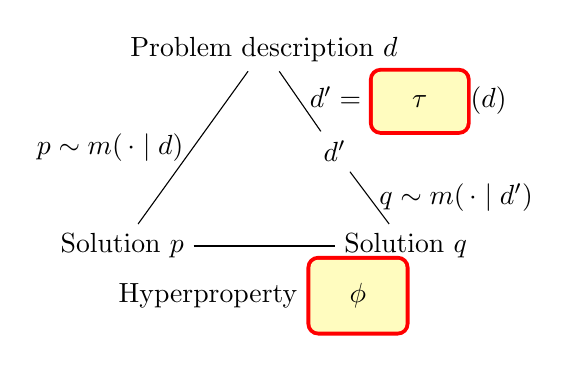
\begin{tikzpicture}[>=stealth, node distance=0.8cm]
        \node (D) at (0,2.5) {Problem description $d$};
        \node (p) at (-1.8,0) {Solution $p$};
        \node (pprime) at (1.8,0) {Solution $q$};
        \node (Dprime) at (0.9,1.2) {$d'$};
        \draw (D) -- (p) node[midway, left] {$p \sim m(\,\cdot \mid d)$};
        \draw (p) -- (pprime) node[midway, below] {Hyperproperty $\hl{\phi}$};
        \draw (D) -- (Dprime) node[midway, right] {$d' = \hl{\tau}(d)$};
        \draw (Dprime) -- (pprime) node[midway, right] {$q\sim m(\,\cdot \mid d')$};
      \end{tikzpicture}
      }
      \vspace{-5mm}
    \end{minipage}
  \end{framed}
  
\noindent where by inducing a bijection we mean that there exists a one-to-one correspondence between equivalence classes of programs such that $\phi$ holds exactly for those pairs $(p,q)$ where the class of $p$ is mapped to the class of $q$. Intuitively, this definition can be interpreted as follows:
\begin{itemize}
\item \emph{Error decorrelation through bijection}: A bijective mapping between equivalence classes guarantees that distinct errors in solutions to the original problem are mapped to distinct errors in solutions to the transformed problem. Consequently, the probability that two independently generated incorrect programs match exactly under a dissociative transformation is low.
\item \emph{Correctness-coupling}: The requirement that the bijection preserves correctness increases the probability of correctness under agreement via $\phi$ since in well-trained models the probabilities of correct solutions are, on average, higher than that of arbitrary bugs.
\end{itemize}

We theoretically justify this definition using a mathematical model tailored to LLM hallucinations. In particular, to capture LLM's lack of genuine understanding of the problem's semantics, which is supported by empirical evidence~\cite{bender2021dangers,shani2025tokens}, we posit that for any given problem, there exists a semantically different problem that the model cannot distinguish (Assumption~\ref{assume:parrot}). Furthermore, drawing on empirical findings of widespread error correlation~\cite{kim2025correlated}, we assume that the LLM produces solutions with imbalanced distributions over equivalence classes of errors (Assumption~\ref{assume:correlated}). Under these assumptions, and using the rearrangement inequality~\cite{hardy1952inequalities}, we prove that an appropriately designed triangulation strictly improves upon plurality voting (Proposition~\ref{prop:triangulation_vs_plurality} and Proposition~\ref{prop:triangulation_vs_plurality_easy}):
\begin{equation*}
\mathds{E}_{d\sim\mathrm{Unif}(D)} \bigl[ \mathds{P}(p\text{ is correct w.r.t. }d \mid \phi(p, q')) - \mathds{P}(p \text{ is correct w.r.t. }d \mid p \equiv q) \bigr] > 0,
\end{equation*}
where $p$ and $q$ are independently sampled solutions for a uniformly chosen problem, $q'$ is a sampled solution to the transformed problem, and $\equiv$ is semantic program equivalence.

\subsection{Inversion-Based Dissociative Problem Transformation}
\label{sec:enum_sinv_example}

Semantic triangulation requires that its problem transformation $\tau$ is dissociative, meaning it changes the task sufficiently that the model does not precisely associate it with the original. Since deriving such a transformation directly from the model weights is infeasible given the complexity of modern LLMs, we instead design it based on intuition and validate the design empirically (\Cref{sec:rq1}).


%% \begin{wrapfigure}{r}{0.45\textwidth}
%%   \vspace{-2mm}
%%   \includesvg[width=0.45\textwidth,pretex=\relscale{0.7}]{elephant.svg}
%%   \vspace{-6mm}
%%   \caption{The parable of the blind men and an elephant illustrates the intuition that hallucinations are not consistent across problem inversions.\label{fig:elephant}}
%%   \vspace{-3mm}
%% \end{wrapfigure}

%% A natural candidate for a dissociative transformation is problem inversion, whose intuition can be illustrated using the ancient Indian parable of the blind men and an elephant (\Cref{fig:elephant}). In the parable, multiple observers each perceive only part of the elephant and draw inconsistent conclusions — e.g., two may describe it as a ``tree'' while one says ``elephant,'' resulting in the plurality forming a false consensus. Imagine now that the elephant is flipped; two may describe it as a ``wall'' while one says ``upside-down elephant,'' again resulting in an erroneous plurality. Crucially, only the third observer's answers remain consistent across both views, while the others' descriptions---rooted in superficial features rather than true understanding---contradict each other. In the context of programming problems, an inverse problem will likely require a fundamentally different algorithm, e.g. a parsing algorithm is substantially different from that of a printer for the same format, making perfectly matching mistakes in their implementations less likely.


\begin{figure}[t]
  \centering
  \includesvg[width=\textwidth,pretex=\relscale{0.75}]{enumsinv.svg}
  \caption{\toolName transforms the program $d$ into two derived problems: $d^{\prec}$, which enumerates all valid outputs for a given input, and $d^{\succ}$, which computes all second-argument values that produce a given output under a given first argument. It then triangulates candidate solutions to $d^{\prec}$ against those to $d^{\succ}$ via ENUM-SINV, identifying a reliable enumerator $e_1$, which is used to discard buggy $p_1$, and select correct $p_2$ via FWD-ENUM.\label{fig:enumsinv}}
  \vspace{-4mm}
\end{figure}%


A natural candidate for a dissociative transformation is problem inversion, since an inverse problem will likely require a different algorithm, e.g. a parsing algorithm is substantially different from that of a printer for the same format, making perfectly matching mistakes in their implementations less likely. However, the challenge of applying problem inversion in practice is that many problems are hard to invert. Formally, inverting a function requires it to be bijective, while most practical problems require implementing non-bijective functions (e.g., squaring is not bijective since both $2$ and $-2$ map to $4$). Although this can be addressed by returning all values that map to a given output, the approach has two limitations. First, a full inversion, e.g., enumerating the values of both $s$ and $t$ for the problem in \Cref{fig:problem}, is often intractable. Second, inexact problems further exacerbate the situation: since multiple valid solutions exist, any concrete solution will fail a bijection-inducing check with a correct inverse, which is a requirement of semantic triangulation (see \Cref{sec:inexact}).


Our tool \toolName identifies the low-probability correct solution $p_2$ and discards the dominant error $p_1$ shown in \Cref{fig:problem}. Initially, it uses an LLM to automatically transform the original problem $d$ into two derived problems shown in \Cref{fig:enumsinv}: an \emph{answer enumeration problem} $d^{\prec}$ and a \emph{set-valued partial inverse problem} $d^{\succ}$. Considering that $d$ is an inexact problem, an enumerator $e$ solving $d^{\prec}$ must, for a given input \mintinline{Python}{e("??", "a")}, return all valid substitutions satisfying the requirements of $d$: \mintinline{Python}{["aa", "ab", ...]}. The set-valued partial inverse $d^{\succ}$ flips the roles of the second argument $t$ and the return value, requiring the computation of all second-argument values that produce a given output under a given first argument. For example, given input \mintinline{Python}{q("??", "ab")}, an inverse $q$ solving $d^{\succ}$ must produce all $t$ that would require such a substitution: \mintinline{Python}{["a", "b", "ab"]}.

After transforming the problems, \toolName samples candidate solutions to both and proceeds as follows. First, it triangulates enumerators (solutions to $d^{\prec}$) against set-valued partial inverses (solutions to $d^{\succ}$) using the hyperproperty ENUM-SINV shown in \Cref{fig:enumsinv}. Concretely, for each candidate enumerator $e$ and each candidate inverse $q$, ENUM-SINV checks whether the two programs agree: for a sampled input, every output listed by $e$ must map back through $q$ to a set containing the original second argument, and vice versa. Since ENUM-SINV is bijection-inducing, a match can only occur when both $e$ and $q$ implement the exact same underlying input-output relation --- just viewed from opposite directions. In our example, the enumerator $e_1$ and inverse $q_1$ pass this check, while other candidate pairs do not, because their independent errors are inconsistent under inversion. Second, it uses the identified enumerator $e_1$ to check solutions to the original problem using the hyperproperty FWD-ENUM. This hyperproperty simply checks the membership of the output of $p$ in the output of $e$. Since FWD-ENUM holds only for $p_2$, it is returned as the plausible solution, while the dominant error $p_1$ is discarded.

The success of this method stems from a combination of factors. First, the transformations are dissociative: as can be seen in \Cref{fig:problem} and \Cref{fig:enumsinv}, all problems require substantially different algorithms, making it non-trivial to produce perfectly matching bugs across them. Second, in contrast to the Hoare triples in \Cref{fig:problem}, ENUM-SINV is bijection-inducing, which we prove in Lean, meaning it can detect even minor inconsistencies between solutions. Thus, while each problem is solved correctly with low probability, only correct solutions match under the hyperproperties.
  
Crucially, all components of this triangulation scheme play distinct roles:

\begin{itemize}
\item A set-valued partial inverse problem $d^{\succ}$ and ENUM-SINV are needed because FWD-ENUM is not bijection-inducing. Like the Hoare triples in \Cref{fig:problem}, it permits enumerators that output overapproximate sets, resulting in spurious matches. As we show experimentally via an ablation, non-bijection-inducing properties do not confer high reliability.
\item An answer enumeration problem $d^{\prec}$ and FWD-ENUM are needed because solutions to the original problem cannot be directly triangulated against set-valued inverses: since the problem is inexact, a correct solution to $d$ does not map to a single correct solution to $d^{\succ}$, and therefore will fail any bijection-inducing, correctness-coupling property.
\end{itemize}

\section{Background, Notation and Basic Assumptions}
\label{sec:background}

We use $\mathds{P}(\cdot)$ to denote probability and $\mathds{E}[\cdot]$ for expectation. Conditional probability $\mathds{P}(A\mid B)$ represents the probability of $A$ given that $B$ holds. We use $d \sim \mathrm{Unif}(D)$ for uniform sampling. Let $D$ be a space of problem descriptions, $P$ be a space of programs. Let $m$ be a code generation model, and $m(\,\cdot\mid d)$ be a distribution of programs conditioned on the description $d$. We denote programs independently sampled from this distribution as $p, q,...\sim m(\,\cdot\mid d)$. The support of a distribution is the set of all programs with non-zero probability. Let $\equiv$ be the (partial) semantic program equivalence relation~\cite{ciobacua2016language}, $\mathcal{P}/{\equiv}$ be the set of all equivalence classes $[p_1]_{\equiv}, [p_2]_{\equiv}, ...$. Since semantic program equivalence is a classical relation, we omit $\equiv$ when denoting equivalence classes w.r.t this relation, e.g. $[p_1]$. Given $[p]$, we call $p$ its representative. We use $\mathrm{id}_A$ to denote the identity function on the domain $A$.

The plurality method selects a representative of the most probable equivalence class. Formally, if we sample $n>2$ programs $S\triangleq \{p_1, p_2, \dots, p_n\}$, that is, $p_1, p_2, \dots, p_n \sim m(\,\cdot \mid d),$ then plurality will select a program $p^\ast \triangleq \arg\max_{p_i \in S} | [p_i] \cap S|$.  This method captures the intuition that a well-trained model assigns higher probability to semantically correct solutions. Random sample consensus (RANSAC)~\cite{fischler1981random} is a classical algorithm designed to detect outliers, which was adapted to eliminate hallucinated program-test pairs in CodeT~\cite{chen2022codet}. In this context, this algorithm is applied to sets of programs $\{p_1, ..., p_n\}$ and witnesses $\{q_1, ..., q_n\}$ to maximize $|P_\mathrm{a}| \cdot |Q_\mathrm{a}|$ where all program in $P_\mathrm{a}$ agree with all witnesses in $Q_\mathrm{a}$. Importantly, plurality is a special case of RANSAC consensus, where equivalence between two programs directly corresponds to their agreement.

The modulus of an array $x$ indexed by $I$ is defined as $\|x\|_{\ell^2(I)}\triangleq\sqrt{\sum_{i\in I}x_i^2}.$

Since prompts are written in natural language, they are prone to imprecision and ambiguity, often allowing conflicting interpretations~\cite{jia2025automated}. We categorize causes of this uncertainty into two groups. We say that a problem description is \emph{ambiguous} if it admits unintended interpretations. For example, in the task ``find three distinct elements of a given list that sum to zero'', the term ``distinct'' may refer either to distinct indices or to distinct values, and it is likely to be a fault in the description. In contrast, a problem description is \emph{inexact} if it omits unimportant details. For example, the specification ``return a positive element of a given list'' allows one to choose a positive element arbitrarily, which is likely valid and even desirable. Indeed, Quan et al.~\cite{quan2025codeelobenchmarkingcompetitionlevelcode} found that even in programming contests, where descriptions are more precise than in typical user prompts, ``about 30\% of problems do not have unique correct outputs.'' We rely on the following assumption:

\begin{assumption}\label{assumption:inexact}
  All descriptions $D$ are unambiguous, but some are inexact.
\end{assumption}

\noindent This relaxes assumptions of previous works. For example, the uncertainty measure by Valentin et al.~\cite{valentin2025estimating} assumes that ``if two LLM-generated programs behave differently on the same input, at least one must be incorrect'', thus requiring prompts that are both unambiguous and exact.

Following standard practice in program verification, we model programs as mathematical functions (please see \Cref{sec:threats} for practical implications):

\begin{assumption}\label{assumption:pure}
  Relevant behavior of solutions to $D$ can be represented as mathematical functions $p: I \rightarrow O$, where $I$ is a space of program inputs, and $O$ is a space of program outputs. 
\end{assumption}

\begin{definition}[Semantic Program Equivalence]
  Programs $p$ and $q$ operating on the same domains are semantically equivalent, which is denoted as $p \equiv q$, iff $\forall i\in I.\ p(i) = q(i).$
\end{definition}

\noindent Given that (partial) program equivalence is undecidable, we estimate it by comparing programs' outputs on LLM-generated inputs provided that the programs terminate within a timeout.

We rely on the existence (without requiring explicit knowledge) of a semantic function $\llbracket \cdot \rrbracket : \mathrm{NL} \to 2^{I \times O}$ that for each problem description returns the required relation between inputs and outputs. For example, $\llbracket ``\text{multiply two numbers}" \rrbracket = \{ ((2, 2), 4), ((2, 3), 6), \cdots \}.$ Inexactness is defined as

\begin{definition}[Exactness]\label{def:exact}
  A problem description $d$ is \emph{exact} if and only if for any $i\in I$, $o, o'\in O$, $(i, o) \in \llbracket d \rrbracket \wedge (i, o') \in \llbracket d \rrbracket \Rightarrow o = o';$ Otherwise, it is \emph{inexact}.
\end{definition}

\begin{example}[Inexact Problem Description]
  \begin{align*}
    \llbracket ``\text{return}\text{ a positive element of a given set}" \rrbracket =\ \{\ &(\{1, -1, 3\}, {\color{red} 1}),\ (\{1, -1, 3\}, {\color{red} 3}), \cdots \}.
  \end{align*}
\end{example}

To simplify our definitions, we assume that all inputs are valid and all outputs are reachable:
\[
\forall i\in I\ \exists o\in O.\ (i, o) \in \llbracket d \rrbracket,\quad \forall o\in O\ \exists i\in I.\ (i, o) \in \llbracket d \rrbracket.
\]
In practice, identifying valid inputs is undecidable; \Cref{sec:implementation} discusses our practical mitigation.

\begin{definition}[Program Correctness w.r.t. Problem Description]\label{def:program_correctness}
  A program $p\in P$ is \emph{correct} w.r.t. a problem description $d\in D$ iff $\forall\ i\in I. (i, p(i)) \in \llbracket d \rrbracket,$ which is denoted as $p \vdash \llbracket d \rrbracket.$ It is \emph{incorrect} iff $\exists i\in I. (i, p(i)) \notin \llbracket d \rrbracket,$ which is denoted as $p \nvdash \llbracket d \rrbracket.$
\end{definition}

Hoare logic~\cite{hoare1969axiomatic} is a framework for specifying expected program behavior. Its central construct, the Hoare triple $\{p\}\;c\;\{q\}$, expresses that, if the program $c$ starts in a state satisfying the precondition $p$, then --- assuming termination --- it will end in a state satisfying the postcondition $q$. Pre- and postconditions are predicates over program states --- mappings from variables to values --- typically expressed in first-order logic~\cite{filliatre2013why3}. Since we assume that programs are pure functions and all inputs are valid, such specifications reduce to $\{\mathrm{True}\}\;o=f(i)\;\{q(i,o)\}$, determined by postconditions $q$.

%% Then, we define correctness of a specification as

%% \begin{definition}[Specification Correctness w.r.t. Problem Description]\label{def:spec_correctness}
%%   A postcondition $q$ is \emph{correct} w.r.t. a problem description $d\in D$ iff $\forall i\in I\ \forall o\in O.\ (i, o) \in \llbracket d \rrbracket \Leftrightarrow q(i, o).$
%% \end{definition}

% While in practice formal specification often overapproximates correct behaviours, focusing on aspects relevant to the user, we require the predicate $q$ to capture the exact set of correct outputs, since in the context of autoformalization, it is unclear how to determine which parts of the requirements are essential for verification and which can be ignored.

\section{Theoretical Basis of Triangulation}
\label{sec:theory}

This section formally justifies the design of semantic triangulation (\Cref{def:triangulation}), along with providing a conceptual account of the underlying improvement. Plurality, test generation, and autoformalization can be unified under the concept of plausibility witnesses. Let $p\sim m(\,\cdot\mid d)$ be a program generated for a description $d$. Suppose there exists a procedure for sampling artifacts $q$ and a criterion ``$\mathrm{agree}$'' for assessing their agreement with $p$. We call such $q$ plausibility witnesses. Based on agreeing pairs $(p, q)$, algorithms such as RANSAC form consensus over the entire sample, and plurality voting is a special case of this algorithm. Thus, a fundamental question arises:

\begin{definition}[Confidence-Enhancing Plausibility Witness Problem]\label{def:witness_problem}
  For a sampled program $p$, what type of plausibility witness $q$ and the corresponding agreement criterion provide higher $\mathds{P}(p\vdash \llbracket d \rrbracket \mid \mathrm{agree}(p, q)),$ the probability that the program is correct under an agreement?
\end{definition}

\subsection{Semantic Triangulation Provably Enhances Confidence Under Agreement}

We prove that triangulation yields higher-confidence witnesses than plurality in a mathematical model of LLM hallucinations, which rigorously explains the mechanism of mitigating hallucinations, informing our practical implementation. To streamline the formal analysis, we adopt several simplifying conventions that
  do not restrict the practical applicability of our approach:
\begin{itemize}
\item to avoid modeling linguistic variations, all descriptions in $D$ are semantically distinct;
\item to facilitate equivalence checking, all programs $P$ operate on exactly the same domains;
\item there is a finite number of equivalence classes $[p_1], [p_2], \cdots, [p_n]$ in $P/\equiv$;
\item the existence of $\phi$ does not require a closed-form representation.
\end{itemize}

Plurality voting operates under the assumption that each problem has a single solution. Indeed, if there are multiple correct solutions to a problem, plurality may prefer high-probability errors even if the total probability mass of all correct solutions is higher. Since our theoretical justification involves a comparison with plurality, in this section we assume that each $d$ has exactly one solution. In the subsequent section, we show how triangulation alleviates this limitation in practice.

Intuitively, triangulation yields higher-confidence witnesses than plurality by mitigating correlated errors. This arises because LLMs, as ``stochastic parrots,'' lack precise semantic understanding and therefore fail to preserve errors under non-trivial transformations. To formalize this intuition, inspired by work on spurious correlations~\cite{ye2024spurious}, we assume that LLMs rely on shallow features preventing them from capturing subtle aspects of problem semantics. At the same time, when a model lacks the ability to discriminate between any problem instances, confidence improvement becomes infeasible. The following assumption reflects these intuitions:

\begin{assumption}[Stochastic Parrots]\label{assume:parrot}
  Let $m$ be a model that defines a distribution of programs conditioned on problem descriptions $m(p \mid d)$. We say that $m$ is a stochastic parrot if for any description $d$, there is a description $d'$ such that $m(\,\cdot \mid d) = m(\,\cdot \mid d')$ and $\llbracket d \rrbracket \neq \llbracket d' \rrbracket$, and a description $d''$ such that $m(\,\cdot \mid d) \neq m(\,\cdot \mid d'')$ and $\llbracket d \rrbracket \neq \llbracket d'' \rrbracket$.
\end{assumption}

\noindent If $m$ is a stochastic parrot, the equivalence relation $\simeq$ defined as $d \simeq d' \Leftrightarrow m(\,\cdot\mid d) = m(\,\cdot\mid d')$ partitions $D$ into at least two equivalence classes containing at least two elements each. We refer to this partitioning $D/\simeq$ as the \emph{hallucination pattern} of $m$.

To formalize the notion of correlated errors, we say that all programs in the same incorrect equivalence class have the same errors, while different classes have different errors. Then, correlated errors across samples for a given problem effectively mean that some equivalence classes are more likely than others. For simplicity, assume that all error classes have different probabilities:

\begin{assumption}[Correlated Errors]\label{assume:correlated}
Let $m$ be a model that defines a distribution of programs conditioned on problem descriptions $m(p \mid d)$. We say that its errors correlate if for each $d$, all classes of programs incorrect w.r.t. $d$ have different probabilities.
\end{assumption}

In our proof, we transform problems by exploiting the hallucination pattern of a stochastic parrot. We pose a requirement for triangulation that it must not make problems arbitrarily harder to solve, i.e., the probabilities of correct solutions for the original problem $d$ and the transformed problem $d'$ must differ from each other less than the probabilities of errors. In the first proposition, operating under a weak \Cref{assume:correlated} that merely establishes that the probabilities of errors are different, we assume that the probabilities of correct solutions to $d$ and $d'$ are the same\footnote{This assumption will be relaxed in \Cref{prop:triangulation_vs_plurality_easy}}:

\begin{figure}[t]
  \centering
  \hspace{8mm}\includesvg[width=0.75\textwidth,pretex=\relscale{0.75}]{rearrangement.svg}
  \caption{Plurality suffers from correlated errors. Triangulation rearranges the mapping of programs to their witnesses so that large classes of program errors are matched with small classes of witness errors and vice versa, which decreases the probability of matching bugs as per the rearrangement inequality.\label{fig:rearrangement}}
\end{figure}%

\begin{proposition}\label{prop:triangulation_vs_plurality}
Let a code generation model $m$ be a stochastic parrot with correlated errors that hallucinates on problems with equal probability of correct solutions. There exists semantic triangulation $(\tau, \phi)$ such that for $p, q\sim m(\,\cdot\mid d)$ and $q'\sim m(\,\cdot\mid \tau(d)),$
  \begin{equation}\label{eq:triangulation_vs_plurality}
    \mathds{E}_{d\sim\mathrm{Unif}(D)} \bigl[ \mathds{P}(p \vdash \llbracket d \rrbracket \mid \phi(p, q')) - \mathds{P}(p \vdash \llbracket d \rrbracket \mid p \equiv q) \bigr] > 0.
\end{equation}
\end{proposition}

\begin{proof}

We construct $\tau$ so that it exploits the stochastic parrot assumption. For each $[d]_\simeq$ in the $m$'s hallucination pattern, we define $\tau$ as a permutation on $[d]_\simeq$ that has no fixed-points.

Let $\phi \triangleq \{ (p, q) \mid d\in D, p \vdash \llbracket d \rrbracket, q \vdash \llbracket \tau(d) \rrbracket \}.$ Since $\tau$ is a permutation on semantically distinct problems, $\phi$ induces a permutation on equivalence classes $[p_1], [p_2], \cdots, [p_n]$. We represent this permutation on the indices $\{1, ..., n\}$ as $\sigma$. By construction, $\phi$ is correctness-coupling, i.e. if $[p_c]$ is correct w.r.t. $d$, then $[p_{\sigma(c)}]$ is correct w.r.t. $\tau(d)$. Therefore, $(\tau, \phi)$ is semantic triangulation. Apart from that, since $\tau$ has no fixed-points, therefore $\sigma$ has no fixed-points. The effect of this permutation $\sigma$, induced by $\phi$, is illustrated in \Cref{fig:rearrangement} using dashed arrows.

Let $\pi_i \triangleq \mathds{P}(p \in [p_i]),$ for $p \sim m(\,\cdot \mid d).$ We can rewrite $\mathds{P}(p \vdash \llbracket d \rrbracket \mid p \equiv q)$ and $\mathds{P}(p \vdash \llbracket d \rrbracket \mid \phi(p, q'))$ as $\frac{\pi_c^2}{\sum\limits_{i}\pi_i^2},$ and $\frac{\pi_c \pi_{\sigma(c)}}{\sum\limits_{i}\pi_i \pi_{\sigma(i)}},$ respectively. Assume $C_d$ are the indices of correct solutions to problems in $[d]_\simeq$, and $B_d$ are the remaining indices of buggy solutions. Then, the expectation in \Cref{eq:triangulation_vs_plurality} for each class $[d]_\simeq$, which we refer to as $\mathds{E}_{d\sim\mathrm{Unif}([d]_\simeq)}(\Delta \mathds{P})$, is expressed as
\begin{equation}\label{eq:delta_elaborated}
\mathds{E}_{d\sim\mathrm{Unif}([d]_\simeq)} \Biggl[ \frac{\pi_c \pi_{\sigma(c)}\sum\limits_{i}\pi_i^2 - \pi_c^2 \sum\limits_{i}\pi_i \pi_{\sigma(i)}}{\sum\limits_{i}\pi_i^2\cdot\sum\limits_{i}\pi_i \pi_{\sigma(i)}} \Biggr] = \frac{\sum\limits_{c\in C_d} \pi_c \pi_{\sigma(c)}\cdot\sum\limits_{i}\pi_i^2 - \sum\limits_{c\in C_d} \pi_c^2 \cdot \sum\limits_{i}\pi_i \pi_{\sigma(i)}}{| [d]_\simeq | \sum\limits_{i}\pi_i^2\cdot\sum\limits_{i}\pi_i \pi_{\sigma(i)}}
\end{equation}

The reduction of correlated errors through triangulation can be explained by the rearrangement inequality~\cite{hardy1952inequalities}. This inequality captures the principle that matching large terms with large terms and small terms with small terms maximizes the sum of products. Specifically, for any real numbers $\pi_1, \pi_2, \dots, \pi_n$ and any permutation $\sigma$, $\sum_{i=1}^n \pi_i^2 \ \ge\ \sum_{i=1}^n \pi_i \pi_{\sigma(i)}$. Moreover, if all $\pi_i$ are different and $\sigma$ has no fixed points, the inequality is guaranteed to be strict.

In our case, $\sigma$ does not preserve any index by construction, and all $\pi_b$ for $b\in B_d$ are distinct due to \Cref{assume:correlated}. Apart from that, since $\sigma$ is a permutation on $[1..n]$ and on $C_d$, therefore it is also a permutation on $B_d$, which contains at least two elements due to \Cref{assume:parrot}. Therefore, for the top part of \Cref{eq:delta_elaborated}, after canceling repeated terms, the following holds:
\begin{equation*}
\sum\limits_{c\in C_d} \pi_c \pi_{\sigma(c)}\cdot \hl{\sum\limits_{b \in B_d}\pi_b^2} - \sum\limits_{c\in C_d} \pi_c^2 \cdot \sum\limits_{b \in B_d}\pi_b \pi_{\sigma(b)} > \sum\limits_{c\in C_d} \pi_c \pi_{\sigma(c)}\cdot\hl{\sum\limits_{b \in B_d}\pi_b \pi_{\sigma(b)}} - \sum\limits_{c\in C_d}\pi_c^2\cdot\sum\limits_{b\in B_d}\pi_b \pi_{\sigma(b)}
\end{equation*}
Since we assumed that all correct solutions to problems in $[d]_\simeq$ have equal probabilities, the RHS of this inequality is zero, therefore $\mathds{E}_{d\sim\mathrm{Unif}(D)}(\Delta \mathds{P}) > 0$.
\end{proof}

The proof of this proposition highlights the interplay between the definition of semantic triangulation (\Cref{def:triangulation}) and our assumptions (\Cref{assume:parrot}, \Cref{assume:correlated}):
\begin{itemize}
\item Bijective mapping reduces the chance of matching errors, as per the rearrangement inequality.
\item Correctness-coupling enables us to exploit the assumption that probabilities of correct samples are not arbitrarily low in well-trained models.
\item The stochastic parrot assumption ensures that errors are not preserved across transformations, and, in combination with correlated errors, makes the rearrangement inequality strict.
\end{itemize}

The preceding proof constructs $\tau$ such that the transformed problem instances are equally difficult to solve as the originals, where ``difficulty'' is defined as the probability of sampling a correct solution. This contrasts with our empirical observations, in which non-semantics-preserving transformations may increase task difficulty. To reconcile this, we introduce the dissociative hallucination pattern assumption that enables us to construct $\tau$ in such a way that it does not make problems significantly harder, while still preventing the model from precisely associating their semantics:

\begin{assumption}[Dissociative Hallucination Pattern]\label{assume:easy_pattern}
  Let $m$ be a stochastic parrot, $D/\simeq$ be its hallucination pattern, $[p_i] \in P/\equiv$ be all program equivalence classes, $c\in C_d$ be all indexes such that $[p_c]$ is correct w.r.t. at least one problem in $[d]_\simeq$, $B_d$ be the remaining indexes, and $\pi_i \triangleq \mathds{P}(p \in [p_i]).$ We say that $D/\simeq$ is dissociative if there exists $\tau$ defined as a permutation on each $[d]_\simeq$, with $\sigma$ being the corresponding permutation on the indexes of a correct solution induced by $\tau$, that the normalized difference between probabilities of correct solutions for the original programs and correct solutions for the transformed problems is lower than difference between probabilities of corresponding errors:
\begin{equation}
 \sum_{c\in C_d}\left(\frac{\pi_c-\pi_{\sigma(c)}}{\|\pi\|_{\ell^2(C_d)}}\right)^2
<\sum_{b\in B_d}\left(\frac{\pi_b-\pi_{\sigma(b)}}{\|\pi\|_{\ell^2(B_d)}}\right)^2
\end{equation}
\end{assumption}

\noindent The justification of this assumption is that if a well-trained model does not distinguish between two problems and produces high-probability bugs, we can still expect that the probabilities of correct solutions to these problems in the distribution should not vary as much as probabilities of errors. Under this assumption, we can prove a more general statement:

\begin{proposition}\label{prop:triangulation_vs_plurality_easy}
Let the model $m$ be a stochastic parrot with a dissociative hallucination pattern. There exists semantic triangulation $(\tau, \phi)$ such that for $p, q\sim m(\,\cdot\mid d)$ and $q'\sim m(\,\cdot\mid \tau(d)),$
  \begin{equation*}
    \mathds{E}_{d\sim\mathrm{Unif}(D)} \bigl[ \mathds{P}(p \vdash \llbracket d \rrbracket \mid \phi(p, q')) - \mathds{P}(p \vdash \llbracket d \rrbracket \mid p \equiv q) \bigr] > 0.
\end{equation*}
\end{proposition}

\begin{proof}
Continuing the derivation for $\mathds{E}_{d\sim\mathrm{Unif}([d]_\simeq)}(\Delta \mathds{P})$ in \Cref{eq:delta_elaborated} leads to the equation in \Cref{assume:easy_pattern}, as elaborated in \Cref{sec:proof_prop_general}.
\end{proof}

%We note that the above assumption do not need not hold for every problem --- it suffices that they hold for a non-trivial fraction of problems, since our guarantees are stated in expectation over uniformly chosed problems.

%% {\color{blue} [UNDER-CONSTRUCTION: MIND YOUR STEP! PEICHU.]}

%% Recall that $C_d=\{1,\cdots,r\}$ and $B_d=\{r+1,\cdots,n\}$. 

%% In general, the hallucination pattern of an LLM can be very complex, and depends on a lot of relevant parameters. To facilitate our quantitative analysis one step forward, some practical assumptions must be made. In particular, we model the buggy classes' occurrence rate in each conditioned probability $m(\cdot|d)$ as a white noise spread over an \emph{effective hallucination range} denoted $n=n(d)$. In other words, the vectors $\pi^B=(\pi_i)_{i\in B_d}$ and $\sigma^B=(\sigma_i)_{i\in B_d}$ are sampled uniformly subject to normalization conditions: $\sum_{i\in B_d}\pi_i=\pi_{bug}$ and $\sum_{i\in B_d}\sigma_i=\sigma_{bug}$ respectively, where $\pi_{bug}=1-\sum_{i\in C_d}\pi_i$, \emph{resp.} $\sigma_{bug}=1-\sum_{i\in C_d}\sigma_i$ (dependent on $[d]_{\simeq}$ implicitly)

%% In general, a larger range $n$ means the hallucination has a messier (in particular, less concentrated) pattern, though individual bug classes may still possess a probability share that is large enough to trouble traditional methods like plurality.

%% \begin{proposition}
%%     If each ambiguity class $[d]_{\simeq}=\{d_1,\cdots,d_r\}$ (success rates $\pi_i=\mathds{P}_{p\sim m(\cdot|d)}(p\vdash\llbracket d_i\rrbracket)$ where $i\in C_d$, noise classes with rates $\pi_i$ where $i\in B_d$) and their inverses $[\check{d}]_{\simeq}=\{\check{d}_1,\cdots, \check{d}_r\}$ (success rates $\sigma_i\ (i\in C_d)$ and noise rates $\sigma_i\ (i\in B_d)$ accordingly) satisfies the following conditions:

%%     (i) For any correct $i\in C_d=\{1,\cdots,r\}$, the inverse problem $\check{d}_i$ is by $\epsilon$ no harder than $d_i$, that is, $\sigma_i\geq (1-\epsilon)\pi_i$.

%%     (ii) The effective hallucination range $n\geq n_0$. The total bug rates $\pi_{bug}$ and $\sigma_{bug}$ satisfy (...)

%%     Then we have
%%     \[
%%     \mathbb E_{d,\pi^B,\sigma^B}\left[\mathds{P}(Failed\ Plurality)-
%%     \mathds{P}(Failed\ Triangulation)\right]>...
%%     \]
%%     where the randomness comes from not only the samples taken (as in previous propositions), but also from the agnostic hallucination pattern.
%% \end{proposition}


%% \begin{proposition}\label{prop:bound}
%% Let $C_1, \dots, C_N$ be outcomes of a discrete distribution $D$ with probabilities
%% \[
%% p_i := P(C_i) > 0, \quad \sum_{i=1}^N p_i = 1,
%% \]
%% and let $f: \{C_1, \dots, C_N\} \to \{C_1, \dots, C_N\}$ be a bijection (permutation) satisfying $f(C_1) = C_2$.
%% {\color{blue} Assume $p_1, p_2, \dots, p_n$ satisfy $p_1\geq\frac{2}{\sqrt{N}}$ and $p_2\geq0.75 p_1$.}
%% Let $a,b$ be independent draws from $D$.
%% Then
%% \[
%% \mathbb E_{f\sim\mathbf{unif}[f(C_1)=C_2]} [\Delta P]\geq11\%,
%% \]
%% where
%% \[
%% \Delta P := P(a \neq C_1,\, b \neq C_1 \mid a = b)-P(a \neq C_1,\, b \neq C_2 \mid b = f(a))
%% \]
%% denotes the fail-rate reduced by adopting triangulation.
%% \end{proposition}

%% \begin{proof}
%% Denote 
%% \[
%% A := \sum_{i=1}^N p_i^2, 
%% \quad B := \sum_{i=1}^N p_i\, p_{f(i)}.
%% \]
%% The first probability is:
%% \[
%% P(a \neq C_1,\, b \neq C_1 \mid a = b)
%% = \frac{\sum_{i \neq 1} p_i^2}{\sum_{i=1}^N p_i^2}
%% = \frac{A - p_1^2}{A}
%% = 1 - \frac{p_1^2}{A}.
%% \]
%% For the second probability, the condition $b = f(a)$ forces $(a,b) = (C_i, f(C_i))$ for some $i$.
%% The restriction $a \neq C_1$ removes $i=1$ from the sum; there is no further removal because $f(C_1) = C_2$ is the only preimage of $C_2$ under $f$.
%% Thus:
%% \[
%% P(a \neq C_1,\, b \neq C_2 \mid b = f(a))
%% = \frac{\sum_{i \neq 1} p_i \, p_{f(i)}}{\sum_{i=1}^N p_i \, p_{f(i)}}
%% = \frac{B - p_1 p_{f(1)}}{B}
%% = \frac{B - p_1 p_2}{B}
%% = 1 - \frac{p_1 p_2}{B}.
%% \]

%% Taking difference of the two probabilities and we get
%% \[
%% \Delta P=\frac{p_1 p_2}{B}-\frac{p_1^2}{A},
%% \]
%% in which only $B$ depends on the random variable $f$. For this purpose we notice that:

%% \[
%% A-B=\frac{1}{2}\sum_{i=1}^N\left(p_i-p_{f(i)}\right)^2,
%% \]

%% by taking expectation {\color{blue} (counting how many times this $i$ connects to that $j$, or something like that)},

%% \[
%% \mathbb E_{f\sim\mathbf{unif}[f(C_1)=C_2]} [B]=A-G,
%% \]

%% where

%% \begin{eqnarray*}
%% G&=&\frac{1}{2(n-1)}\cdot\left[n(p_1-p_2)^2+\sum_{i=3}^N((p_1-p_i)^2+(p_2-p_i)^2)\right.\\
%% &&\left.
%% \ \ \ \ \ \ \ \ \ \ \ \ 
%% \ \ \ \ \ \ \ \ \ \ \ \ 
%% \ \ \ \ \ \ \ \ \ \ \ \ 
%% \ \ \ \ \ \ \ \ \ \ \ \ 
%% +2\cdot{\sum_{3\leq\ i<j\ \leq N}}(p_i-p_j)^2\right]\\
%% &=&(calculation-omitted)\\
%% &=&A-p_1p_2-\frac{1}{N-1}(1-p_1)(1-p_2)
%% \end{eqnarray*}

%% \begin{eqnarray}
%% &&\mathbb E_{f\sim\mathbf{unif}[f(C_1)=C_2]} [\Delta P]\\
%% &=&\mathbb E_{f\sim\mathbf{unif}[f(C_1)=C_2]} \left[\frac{p_1 p_2}{B}-\frac{p_1^2}{A}\right]\\
%% &\geq&\frac{p_1 p_2}{\mathbb E_{f\sim\mathbf{unif}[f(C_1)=C_2]} [B]}-\frac{p_1^2}{A}\\
%% &=&\frac{p_1 p_2}{A-G}-\frac{p_1^2}{A}\\
%% &=&\frac{1}{1+\frac{1}{N-1}\left(\frac{1}{p_1}-1\right)\left(\frac{1}{p_2}-1\right)}-\frac{p_1^2}{p_1^2+p_2^2+\sum_{j=3}^Np_j^2}\\
%% &\geq&\frac{1}{1+\frac{1}{N-1}\left(\frac{1}{p_1}-1\right)\left(\frac{1}{p_2}-1\right)}-\frac{p_1^2}{p_1^2+p_2^2+\frac{1}{N-2}(1-p_1-p_2)^2}\\
%% \end{eqnarray}

%% {\color{blue} [1. The first $\geq$ is not that loose.] [2. The second $\geq$ is more useful when $p_1,p_2>>p_2,\cdots,p_N$. When several $p_j$ ($j\geq3$) are $\sim p_1,p_2$, we need more.]}

%% If $p_1\geq\frac{\sigma}{\sqrt{N}}$ and $p_2\geq\beta\cdot p_1$ (where $\beta\sigma\geq1$), we further have
%% \begin{eqnarray}
%% &&[above-formula]\\
%% &\geq&\frac{1}{1+\frac{1}{N-1}\left(\frac{\sqrt{N}}{\sigma}-1\right)\left(\frac{\sqrt{N}}{\beta\sigma}-1\right)}-\frac{p_1^2}{p_1^2+(\beta p_1)^2}\\
%% &\geq&\frac{1}{1+\frac{1}{N-1}\frac{\sqrt{N}-1}{\sigma}\frac{\sqrt{N}-1}{\beta\sigma}}-\frac{1}{1+\beta^2}\\
%% &\geq&\frac{1}{1+\frac{1}{\beta\sigma^2}}-\frac{1}{1+\beta^2}\\
%% \end{eqnarray}

%% In particular, if $\sigma=2$ and $\beta=0.75$, then we have $\mathbb E[\Delta P]\geq0.11$, that is, at least an $11\%$ probability gap is \emph{expected} with respect to all relevant permutations.

%% \end{proof}


%% \subsection{Theoretical Comparison with Prior Work}
%% \label{sec:triangulation_vs_autoformalization}

%% If $\tau\triangleq \mathrm{id}_\mathcal{D}$ is the identity transformation, and $\phi\triangleq\ \equiv$ is semantic program equivalence, then triangulation reduces to the plurality method. In this sense, triangulation generalizes plurality. 

%% \begin{proposition}[Triangulation Generalizes Plurality]
%%   $(\mathrm{id}_\mathcal{D}, \equiv)$ is semantic triangulation.
%% \end{proposition}

%% \noindent However, plurality is an ineffective form of triangulation, because an identity transformation does not disrupt error correlations, i.e., does not exploit \Cref{assume:easy_pattern}. 

%% One might suspect that autoformalizing requirements into e.g., Hoare Logic~\cite{hoare1969axiomatic} specifications, constitutes an instance of triangulation. It is easy to show that naive autoformalization, and consequently test generation, are not instances of triangulation, since they lack a bijective mapping between program errors and specification (or test) errors:

%% \begin{proposition}[Naive Autoformalization is Not Triangulation]\label{prop:postcondition_not_triangulation}
%%   Let $(\tau, \phi)$ be such that $\tau$ transforms a coding problem into a problem of generating postconditions, and $\phi$ is a verification tool. Then, $(\tau, \phi)$ is not semantic triangulation.
%% \end{proposition}

%% \begin{proof}
%%   The witness $q\triangleq \mathrm{True}$ agrees with any program, therefore the mapping between equivalence classes of errors induced by $\phi$ is not bijective.
%% \end{proof}

%% \noindent That is, naive autoformalization into Hoare Logic does not disrupt error correlation, because overly-permissive witnesses may agree with many errors in generated programs. As we show empirically (\Cref{sec:evaluation}), this limits its effectiveness in detecting hallucinations.

\section{Practical Design of Triangulation}
\label{sec:practical}

Our practical design of semantic triangulation methods is based on the insights of our theoretical analysis (\Cref{assume:easy_pattern}) that require that the transformed problems are not significantly harder to solve, while it is hard to exactly match errors in their implementations. In particular, we transform a problem into one that requires a different algorithm while still being ``natural'' for an LLM to solve. Our transformations involve algorithm inversion, answer enumeration and problem decomposition. Specifically, we introduce three inversion-based methods consisting of problem transformations and corresponding hyperproperties: FWD-INV, FWD-SINV, and ENUM-SINV, and a meta triangulation method STREAM for stateless stream-processing programs. All transformations are performed automatically by prompting an LLM (see, e.g., \Cref{fig:sinv_transformation_prompt}).

To specify the intended effect of transformations, we use an imaginary procedure $\llparenthesis\ \cdot\ \rrparenthesis$ that, given a binary relation between inputs and outputs, converts it into natural language text.

\begin{definition}[Inverse Problem]
  Let $d$ be a problem such that $\llbracket d \rrbracket\subset I\times O$. The corresponding inverse problem is $d^{-1} \triangleq \llparenthesis\ \{(o, i) \mid (i, o) \in \llbracket d \rrbracket\}\ \rrparenthesis.$
\end{definition}

\begin{proposition}[Full FWD-INV]
  Let $\tau$ transform each problem $d$ into $d^{-1}$, $p$ is a sample for $d$, $q$ is for $d^{-1}$, and $\phi\triangleq q \circ p \equiv \mathrm{id_I} \wedge \forall o, o'\in O.\ o \neq o' \Rightarrow q(o) \neq q(o')$. If $\tau$ is dissociative, then $(\tau, \phi)$ is semantic triangulation (\Cref{def:triangulation}). We refer to this triangulation method as Full FWD-INV.
\end{proposition}

\begin{proof}
  A proof that $\phi$ is bijection-inducing and correctness-coupling is mechanized in Lean.
\end{proof}

Our hypothesis is that inversion-based transformation exploits dissociative hallucination patterns, because forward and inverse problems often require different algorithms. However, fully inverting an algorithm is often infeasible. Consider, for example, the problem ``given a graph and two of its nodes, compute the length of the shortest path between them''. A full inversion would require producing any pair consisting of a graph and two nodes whose shortest-path distance matches a specified value --- such outputs would likely fail to align with the behavior of the original forward algorithm, or else require exhaustively enumerating all such pairs, which is infeasible.

To alleviate this problem, we apply a more natural and practical partial inversion, that is inverting an algorithm w.r.t. a single parameter. For instance, ``given a graph and a target distance, enumerate all pairs of nodes whose shortest-path length is exactly that distance''. This formulation is easier for an LLM to handle, while still satisfying the properties required for semantic triangulation:


\begin{definition}[Partial Inverse Problem]
  Let $d$ be a problem such that $\llbracket d \rrbracket\subset (I_1 \times I_2) \times O$. The corresponding partial inverse problem w.r.t. the first argument is $$d^{-1}_1 \triangleq \llparenthesis\ \{((o, i_2), i_1) \mid ((i_1, i_2), o) \in \llbracket d \rrbracket\}\ \rrparenthesis.$$
\end{definition}

\noindent The inversion with respect to other arguments is defined accordingly. In practice, we prompt an LLM to decide which argument to use for inverting the problem.

\begin{proposition}[Partial FWD-INV]\label{prop:partial_fwd_inv}
  Let $\tau$ transform each problem $d$ into $d^{-1}_1$, and $$\phi\triangleq \forall (i_1, i_2)\in I.\ q(p(i_1, i_2), i_2) = i_1 \wedge\ \forall (o, i_2), (o', \_)\in O'.\ o \neq o' \Rightarrow q(o, i_2) \neq q(o', i_2),$$ where $p$ is a sample for $d$, $q$ is for $d^{-1}_1$ and $O'$ refers to all inputs to $q$. If $\tau$ is dissociative, then $(\tau, \phi)$ is semantic triangulation. We refer to this triangulation method as Partial FWD-INV.
\end{proposition}

\begin{proof}
  A proof that $\phi$ is bijection-inducing and correctness-coupling is mechanized in Lean.
\end{proof}

Although the problem inversion defined above is likely to change the solution algorithms, while keeping the problem tractable for an LLM, its key limitation is that for the hyperproperty to faithfully hold, i.e., hold on pairs of correct solution-witness pairs, the problem description must permit bijective functions as valid solutions. This, however, often does not hold in practice. For example, for the problem ``compute the square of a given number'', a correct solution maps both $-i$ and $i$ to $i^2$, implying that only incorrect forward and inverse implementations will match.

To alleviate this challenge, we employ set-valued inverses that return the exhaustive list of values for a given input argument that would result in a given output:

\begin{definition}[Set-valued Inverse Problem]
  Let $d$ be a problem such that $\llbracket d \rrbracket\subset I\times O$. The corresponding set-valued inverse problem is $$d^{\succ} \triangleq \llparenthesis\ \bigl\{(o, \{i \mid (i, o) \in \llbracket d \rrbracket \}) \mid (\_, o) \in \llbracket d \rrbracket \bigr\}\ \rrparenthesis.$$
\end{definition}

\begin{proposition}[Full FWD-SINV]\label{prop:full_fwd_sinv}
  Let $\tau$ transform each problem $d$ into $d^{\succ}$, and $$\phi\triangleq \forall i \in I.\ \underbrace{i \in q(p(i))}_{L_1} \wedge \underbrace{\forall i' \in q(p(i)).\ p(i') = p(i)}_{L_2} \wedge\ \underbrace{\forall o, o'\in O.\ o \neq o' \Rightarrow q(o) \cap q(o') = \emptyset}_{L_3},$$ where $p$ is a sample for $d$ and $q$ is for $d^{\succ}$. If $\tau$ is dissociative, then $(\tau, \phi)$ is semantic triangulation. We refer to this triangulation method as Full FWD-SINV.
\end{proposition}

\begin{proof}
  Intuitively, a correctness-coupling bijective mapping via $\phi$ is achieved through the interplay of $L_1$, $L_2$, and $L_3$. In particular, $L_1$ ensures that if $p$ is correct, then $q$ never misses a value in its output on the range of $p$, and if $q$ is correct on the range of $p$, then $p$ never returns an incorrect value. In turn, $L_2$ complements $L_1$ by ensuring that if $p$ is correct, then $q$ never returns an incorrect value on the range of $p$. Finally, $L_3$ ensures that $q$ matches the behaviour of a single forward function. A full proof is mechanized in Lean.
\end{proof}

% This proof highlights the necessity to have a coarser relation than $\equiv$ in the definition of semantic triangulation (\Cref{def:triangulation}) --- the above hyperproperty $\phi$ binds the correctness of $p$ on all inputs with the correctness of $q$ only on the range of $p$.

As with FWD-INV, we define a partial version of FWD-SINV:

\begin{definition}[Partial Set-valued Inverse Problem]
  Let $d$ be a problem such that $\llbracket d \rrbracket\subset (I_1 \times I_2) \times O$. The corresponding partial set-valued inverse problem w.r.t. the first argument is $$d^{\succ}_1 \triangleq \llparenthesis\ \bigl\{\bigl((o, i_2), \{i_1 \mid ((i_1, i_2), o) \in \llbracket d \rrbracket \}\bigr) \mid ((\_, i_2), o) \in \llbracket d \rrbracket \bigr\}\ \rrparenthesis.$$
\end{definition}

\begin{proposition}[Partial FWD-SINV]
  Let $\tau$ transform each problem $d$ into $d^{\succ}_1$, and
\begin{align*}
\phi\ \triangleq&\ \forall (i_1, i_2) \in I.\ i_1 \in q(p(i_1, i_2), i_2) \wedge \forall i_1' \in q(p(i_1, i_2), i_2).\ p(i_1', i_2) = p(i_1, i_2)\\
\wedge&\ \forall (o, i_2), (o', \_)\in O'.\ o \neq o' \Rightarrow q(o, i_2) \cap q(o', i_2) = \emptyset,
\end{align*}
where $p$ is a sample for $d$, $q$ is for $d^{\succ}_1$ and $O'$ refers to all inputs to $q$. If $\tau$ is dissociative, then $(\tau, \phi)$ is semantic triangulation. We refer to this triangulation method as Partial FWD-SINV.
\end{proposition}

\begin{proof}
  A proof that $\phi$ is bijection-inducing and correctness-coupling is mechanized in Lean.
\end{proof}

Automating such a transformation with an LLM is straightforward, as it often reduces to a simple linguistic reformulation and does not require the reasoning to actually solve the problem. A fragment of the prompt used for Partial FWD-SINV transformation is given in \Cref{fig:sinv_transformation_prompt}.

\begin{figure}[t]
    \centering
        {\scriptsize
      \begin{tcolorbox}[mybox,title={SINV problem transformation prompt template}]
      \begin{minted}[escapeinside=||]{text}
You are given a programming problem that requires implementing the function {ORIG_SIGN}. Rewrite this problem
so that it instead requires implementing the set-valued inverse function {SINV_SIGN}. Given the desired output
value {NEW_ARG} (corresponding to the original function's return value), the new function should return an
exhaustive list of values for the parameter {INV_ARG} such that if the original function were called with
any of these values (and the other parameters unchanged), it would produce {NEW_ARG} as the result.
      \end{minted}
      \end{tcolorbox}
    }
    \vspace{-4mm}
\caption{\label{fig:sinv_transformation_prompt}A fragment of prompt template used for set-valued inverse problem transformation. \texttt{ORIG\_SIGN} is the typed signature of the original function, \texttt{INV\_SIGN} is the signature of the inverse function, \texttt{NEW\_ARG} is the argument of the inverse function representing the output of the original function, \texttt{INV\_ARG} is the argument for inversion. The argument to invert (\texttt{INV\_ARG}) is chosen by an LLM using a separate prompt.}
\vspace{-3mm}
\end{figure}


\subsection{Triangulation for Inexact Problems}
\label{sec:inexact}

\begin{figure}[t]
    \centering
    \begin{subfigure}[t]{0.32\textwidth}
    {\scriptsize
    % Prompt box
      \begin{tcolorbox}[mybox,title={Original problem $d$}]
Implement \mintinline{python}{p(i: int) -> int} that returns an integer strictly greater than i by at most 2.
      \end{tcolorbox}
    % Response box
      \begin{tcolorbox}[mybox,title=Sample $p$]
        \begin{minted}[escapeinside=||]{python}
def p(i: int) -> int:
  return i+1
        \end{minted}
    \end{tcolorbox}
    }
    \end{subfigure}%
    \hfill
\begin{subfigure}[t]{0.32\textwidth}
    {\scriptsize
    % Prompt box
      \begin{tcolorbox}[mybox,title={Inverse problem $d^{-1}$}]
Implement \mintinline{python}{q(i: int) -> int} that returns an integer strictly smaller than i by at most 2.
      \end{tcolorbox}
    % Response box
      \begin{tcolorbox}[mybox,title=Sample $q$]
        \begin{minted}[escapeinside=||]{python}
def q(i: int) -> int:
  return i-2
        \end{minted}
    \end{tcolorbox}
    }
\end{subfigure}
    \hfill
\begin{subfigure}[t]{0.32\textwidth}
    {\scriptsize
    % Prompt box
      \begin{tcolorbox}[mybox,title={Set-valued inverse problem $d^{\succ}$}]
Implement \mintinline{python}{q(i: int) -> list[int]} that returns all integers strictly smaller than i by at most 2.
      \end{tcolorbox}
    % Response box
      \begin{tcolorbox}[mybox,title=Sample $q'$]
        \begin{minted}[escapeinside=||]{python}
def q(i: int) -> list[int]:
  return [i-1, i-2]
        \end{minted}
    \end{tcolorbox}
    }
\end{subfigure}
\vspace{-3mm}
\caption{\label{fig:inexact_challenge}It is challenging to achieve consensus for problems that permit multiple non-equivalent solutions.}
\end{figure}

Inexact problems permit multiple non-equivalent solutions (\Cref{def:exact}), e.g., the task ``generate a script that extracts all customers from a CSV'' can be interpreted as saving customer data to a file or printing it to stdout, returning it in sorted order or not, and deciding which specific information to extract. Some details are likely irrelevant to the user's goal. We speculate that in practice, most code generation prompts are inexact. In contrast, to the best of our knowledge, existing techniques to establish consensus or control uncertainty, sometimes explicitly~\cite{valentin2025estimating}, assume that only one solution is correct, since forming a consensus under inexact problem descriptions is challenging.

\Cref{fig:inexact_challenge} illustrates this challenge. The original problem admits at least two non‑equivalent solutions: $i \mapsto i+1$ and $i \mapsto i+2$ (for simplicity, we omit solutions whose logic varies depending on the input). This undermines plurality, as the vote may select a high‑probability error even when correct solutions have greater total probability mass. This also hinders the above triangulation methods. For example, composing the inverse program $q$ with the forward program $p$ in \Cref{fig:inexact_challenge} does not yield an identity function as required by FWD-INV, despite both programs being correct individually. Similarly, in the context of FWD-SINV, the clause $\forall i' \in q'(p(i)).\ p(i') = p(i)$ in \Cref{prop:full_fwd_sinv} fails, as for $i=1$, $q'(p(i))$ is $\{0, 1\}$, but $p(0) \neq p(1)$.

Triangulation is the first to alleviate this problem; it generates a program to exhaustively enumerate valid answers for each input, and triangulate this enumerator against a set-valued inverse.

\begin{definition}[Answer Enumeration Problem]
  Let $d$ be a problem such that $\llbracket d \rrbracket\subset I\times O$. The corresponding answer enumeration problem is $$d^{\prec} \triangleq \llparenthesis\ \bigl\{(i, \{o \mid (i, o) \in \llbracket d \rrbracket \}) \mid (i, \_) \in \llbracket d \rrbracket \bigr\}\ \rrparenthesis.$$
\end{definition}

An enumerator is inefficient as a solution to the original problem; to address it, we sample solutions to three problems: the original problem $d$, the enumeration problem $d^{\prec}$, and the set-valued inverse problem $d^{\succ}$. After triangulating a solution to $d^{\prec}$ with a solution to $d^{\succ}$, we triangulate a solution to $d$ with $d^{\prec}$. Note that triangulating with $d^{\succ}$ cannot be omitted, since triangulating only $d$ with $d^{\prec}$ lacks the bijective property of semantic triangulation and therefore does not sufficiently decorrelate errors. We call such a triangulation scheme a \emph{cascade}.

\begin{proposition}[Full ENUM-SINV]\label{prop:full_enum_sinv}
  Let $\tau_1$ transform each problem $d$ into $d^{\prec}$, and $\tau_2$ transform each problem $d$ into $d^{\succ}$. Let a hyperproperty $\phi$ defined as
\[
\forall i \in I.\ \forall o \in p(i).\ i \in q(o) \wedge \forall o \in O.\ \forall i \in q(o).\ o \in p(i)
\]
where $p$ is a sample for $d^{\prec}$ and $q$ is for $d^{\succ}$. If $\tau_2 \circ \tau_1^{-1}$ is dissociative, then $(\tau_2 \circ \tau_1^{-1}, \phi)$ is semantic triangulation. We refer to this triangulation method as Full ENUM-SINV cascade.
\end{proposition}

\begin{proof}
  A proof that $\phi$ is bijection-inducing and correctness-coupling is mechanized in Lean.
\end{proof}

To illustrate this hyperproperty, refer again to \Cref{fig:inexact_challenge}. Assume an incorrect enumerator $p' \triangleq i \mapsto [i+1]$ misses $i+2$ in its output. Although $L_1$ will hold for any input to $p'$, the clause $L_2$ will fail. For example, for $o=2$, $q'(o)$ will return $\{0, 1\}$, but $2\notin p'(0)$. At the second phase, solutions $p$ to $d$ are checked against triangulated enumerators $p''$ via FWD-ENUM: $\forall i\in I.\ p(i) \in p''(i).$

Similar to previous triangulation methods, we define a partial inversion variant of ENUM-SINV:

\begin{proposition}[Partial ENUM-SINV]\label{prop:partial_enum_sinv}
  Let $\tau_1$ transform each problem $d$ into $d^{\prec}$, and $\tau_2$ transform each problem $d$ into $d^{\succ}_1$. Let the hyperproperty $\phi$ be defined as
\[
\forall (i_1, i_2) \in I.\ \forall o \in p(i_1, i_2).\ i_1 \in q(o, i_2) \wedge \forall (o, i_2) \in O'.\ \forall i_1 \in q(o, i_2).\ o \in p(i_1, i_2)
\]
where $p$ is a sample for $d^{\prec}$, $q$ is for $d^{\succ}_1$, and $O'$ refers to all inputs to $q$. If $\tau_2 \circ \tau_1^{-1}$ is dissociative, then $(\tau_2 \circ \tau_1^{-1}, \phi)$ is semantic triangulation. We refer to this method as Partial ENUM-SINV cascade.
\end{proposition}

\begin{proof}
  A proof that $\phi$ is bijection-inducing and correctness-coupling is mechanized in Lean.
\end{proof}

\subsection{Problem Decomposition}

Problems involving non-trivial data structures are hard for LLMs to invert. To simplify inversion, we apply a domain-specific decomposition. In particular, we define a triangulation method STREAM for stateless stream-processing problems, i.e., that process sequences of elements without depending on global state. We designate solutions to such problems $p: \mathrm{Seq}[I] \rightarrow \mathrm{Seq}[O]$. Let $[\cdot]$ be a sequence constructor, $\mathrm{head}: \mathrm{Seq}[I] \rightarrow I$ return the first element of a sequence.

\begin{proposition}[STREAM]\label{prop:stream}
  Let $d$ be a stateless stream-processing problem, $(\tau, \phi)$ be semantic triangulation, $\tau^{\circ}$ transform a stateless stream-processing problem into a corresponding pointwise problem that processes individual elements. Let the hyperproperty $\psi$ be defined as
\[
\phi(p^{\circ}, q) \wedge \forall\ [i_1, \cdots, i_n] \in \mathrm{Seq}[I].\ p([i_1, \cdots, i_n]) = [p^{\circ}(i_1), \cdots, p^{\circ}(i_n)]
\]
where $p$ is a sample for $d$, $p^{\circ}\triangleq i \mapsto \mathrm{head}(p([i]))$. If $\tau$ is dissociative, then $(\tau \circ \tau^{\circ}, \psi)$ is semantic triangulation. We refer to this triangulation meta-method as STREAM.
\end{proposition}

\begin{proof}
  A proof that $\psi$ is bijection-inducing and correctness-coupling is mechanized in Lean.
\end{proof}

\noindent Effectively, STREAM applies a given triangulation method pointwise and then triangulates the lifting from pointwise to sequence-level processing. This demonstrates the modularity of triangulation.

%% TODO: maybe move this to appendix?
%% Furthermore, we apply two type-guided problem decomposition methods. First, we decompose data structures into separate input parameters to simplify inversion. For example, instead of the problem that requires \mintinline{Python}{sum(l: list[int]) -> int}, we invert an equivalent transformed problem requiring \mintinline{Python}{sum(head: Optional[int], tail: list[int]) -> int}, w.r.t. the first parameter \mintinline{Python}{head}, which may be \mintinline{Python}{None} only if \mintinline{Python}{tail} is empty. Additionally, when the required function returns a union type such as \mintinline{Python}{Optional}, we invert the problem w.r.t. each individual type disjunct, and compose sampled solutions as shown in \Cref{fig:motivating}.

\subsection{Implementation}
\label{sec:implementation}

We implemented triangulation in a tool called \toolName for Python programs. To form consensus over the entire sample from individual agreements, we apply RANSAC in a manner similar to CodeT. In addition, we implemented autoformalization into Hoare Logic–style postconditions, expressed as boolean Python functions to avoid limitations of low-resource specification languages.

Formal verification of Python code is hampered by the gap between capabilities of SOTA LLM-based code generation and automated formal verification. Even on simpler benchmarks like HumanEval~\cite{chen2021evaluating} --- where SOTA LLMs nearly solve all tasks --- these LLMs automate verification of correct solutions with the SOTA Python verifier Nagini~\cite{eilers2018nagini} in only 15\% of cases~\cite{shefer2025can}. To obtain enough signal on harder benchmarks, we approximate property validity by testing properties on LLM-generated inputs. We crafted prompts that sample until each problem reaches high coverage, and we use the same input sets for all baselines to ensure fairness.


\begin{figure}[t]
{\scriptsize
\begin{mathpar}
    \inferrule*[right=exec\_s]
    {\langle \Sigma, t \rangle \Rightarrow s}
    {\langle \Sigma, p(t) \rangle \Rightarrow s}

    \inferrule*[right=or\_d]
    {\langle \Sigma, t \rangle \Rightarrow \mathcal{D}}
    {\langle \Sigma, t \vee \_ \rangle \Rightarrow \mathcal{D}}

    \inferrule*[right=or\_a]
    {\langle \Sigma, t_1 \rangle \Rightarrow \mathcal{A} \\
    \langle \Sigma, t_2 \rangle \Rightarrow \overline{\mathcal{D}}}
    {\langle \Sigma, t_1 \vee t_2 \rangle \Rightarrow \mathcal{A}}

    \inferrule*[right=or\_u]
    {\langle \Sigma, t_1 \rangle \Rightarrow \mathcal{U} \\
    \langle \Sigma, t_2 \rangle \Rightarrow ?\\
    ? \notin \{\mathcal{A}, \mathcal{D}\}}
    {\langle \Sigma, t_1 \vee t_2 \rangle \Rightarrow \mathcal{U}}

    \inferrule*[right=eq\_d]
    {\langle \Sigma, t \rangle \Rightarrow \mathcal{D}}
    {\langle \Sigma, t = \_ \rangle \Rightarrow \mathcal{D}}

    \inferrule*[right=eq\_uu]
    {\langle \Sigma, t_1 \rangle \Rightarrow \mathcal{U} \\
    \langle \Sigma, t_2 \rangle \Rightarrow \mathcal{U}}
    {\langle \Sigma, t_1 = t_2 \rangle \Rightarrow \mathrm{True}}

    \inferrule*[right=eq\_a]
    {\langle \Sigma, t_1 \rangle \Rightarrow \mathcal{A} \\
    \langle \Sigma, t_2 \rangle \Rightarrow \overline{\mathcal{D}}}
    {\langle \Sigma, t_1 = t_2 \rangle \Rightarrow \mathcal{A}}

    \inferrule*[right=eq\_u]
    {\langle \Sigma, t_1 \rangle \Rightarrow \mathcal{U} \\
    \langle \Sigma, t_2 \rangle \Rightarrow \overline{s}}
    {\langle \Sigma, t_1 = t_2 \rangle \Rightarrow \mathcal{U}}

    \inferrule*[right=in\_inf]
    {\langle \Sigma, v \rangle \Rightarrow \overline{s}\\
    \langle \Sigma, t \rangle \Rightarrow V^\ast\\
    \overline{s} \in V^\ast}
    {\langle \Sigma, v\in t \rangle \Rightarrow \mathrm{True}}

    \inferrule*[right=in\_inf\_a]
    {\langle \Sigma, v \rangle \Rightarrow \overline{s}\\
    \langle \Sigma, t \rangle \Rightarrow V^\ast\\
    \overline{s} \notin V^\ast}
    {\langle \Sigma, v\in t \rangle \Rightarrow \mathcal{A}}

    \inferrule*[right=in\_uu]
    {\langle \Sigma, v \rangle \Rightarrow \mathcal{U}\\
    \langle \Sigma, t \rangle \Rightarrow \mathcal{U}}
    {\langle \Sigma, v\in t \rangle \Rightarrow \mathrm{True}}

    \inferrule*[right=in\_s]
    {\langle \Sigma, v \rangle \Rightarrow ?_1\\
    \langle \Sigma, t \rangle \Rightarrow ?_2\\
    \{?_1, ?_2\} \cup S \neq \emptyset \wedge \{?_1, ?_2\} \setminus \{\mathcal{U}\} \neq \emptyset}
    {\langle \Sigma, v\in t \rangle \Rightarrow\ \uparrow(\{?_1, ?_2\})}

    \inferrule*[right=forall]
    {\langle \Sigma, t_1 \rangle \Rightarrow \{\overline{s}_i\}_i\\
    \forall i.\ \langle \Sigma[v\mapsto \overline{s}_i], t_2 \rangle \Rightarrow\ ?_i}
    {\langle \Sigma, \forall\ v\in t_1.\ t_2 \rangle \Rightarrow \forall i.\ ?_i \in \{\mathcal{A}, \mathrm{True}\} \wedge |\{?_i\mid ?_i = \mathcal{A}\}_i| < T}

    \inferrule*[right=forall\_s]
    {\langle \Sigma, t \rangle \Rightarrow s}
    {\langle \Sigma, \forall\ v\in t.\ \_ \rangle \Rightarrow s = \mathcal{A}}

\end{mathpar}
}
\vspace{-6mm}
  \caption{Semantics of handling errors and infinite sets during property checking, where $\Rightarrow$ --- the evaluation relation, $\Sigma$ --- a variable assignment, $t$ --- a term, $x$ --- a variable, $S$ --- all special values $\{\mathcal{A}, \mathcal{U}, \mathcal{D}\}$, $s$ --- a special value, $\overline{\mathcal{D}}$ --- any value except for $\mathcal{D}$, $\overline{s}$ --- a non-special value, $V$ --- a finite set of non-special values, $V^\ast$ --- a marked subset of an unknown set of non-special values, $p$ --- a program, $\mathtt{exec}$ --- an execution procedure, $?$ --- any value or set, $\uparrow$ selects the ``strongest'' special value, where $\mathcal{D}$ is stronger than $\mathcal{A}$ and $\mathcal{A}$ is stronger than $\mathcal{U}$, $T$ --- threshold parameter. Logical connectives are handled analogously to $\vee$, all rules respect commutativity.\label{fig:error_handling}. The standard semantics for non-special values is given in appendix (\Cref{fig:normal_handling}).}
  \vspace{-2mm}
\end{figure}

\toolName implements practical mitigations to two fundamental problems: (1) in practice, many inputs are invalid, e.g., negative numbers for Fibonacci, and (2) some transformed problems, e.g., a set-valued inverse, may require enumerating infinite or intractable sets. First, our code-generation prompt instructs programs to validate inputs and raise \texttt{ValueError} on invalid cases following common Python practice. Second, this prompt requests enumerating only a tractable subset when the answer set is infinite or too large, and marking the output accordingly.

\begin{figure}[t]
\centering
\begin{subfigure}[c]{0.45\textwidth}
\centering
\scalebox{0.7}{
\begin{tabular}{cccc}
\toprule
\diagbox{GT}{R} & \makecell{Correctly \\ selected} & \makecell{Incorrectly \\ selected} & Abstained \\
\midrule
No abstention & \cellcolor{lightgreen}\( N_1 \) & \cellcolor{lightred}\( N_2 \) & \cellcolor{lightred}\( N_3 \) \\
Abstention & & \cellcolor{lightred}\( N_4 \) & \cellcolor{lightgreen}\( N_5 \) \\
\bottomrule
\end{tabular}
}
\caption{{\footnotesize Abstention confusion matrix. ``GT'' is the ground-truth, where ``Abstention'' indicates tasks with no correct solutions in the sample; ``R'' is the sample consensus response. When GT is abstention, the response can only be either ``Abstained'' or ``Incorrectly selected''.}}
\label{fig:sub-table}
\end{subfigure}
\begin{subfigure}[c]{0.5\textwidth}
\centering
\footnotesize
\begin{align*}
\text{Reliable Accuracy} &= \frac{N_1}{N_1 + N_2 + N_4} \\
\text{Overall Accuracy} &= \frac{N_1 + N_5}{N_1 + N_2 + N_3 + N_4 + N_5} \\
\text{Abstention Rate} &= \frac{N_3 + N_5}{N_1 + N_2 + N_3 + N_4 + N_5} \\
\end{align*}
\vspace{-2.3\baselineskip}
\begin{gather*}
\text{Precision}_\mathrm{abs} = \frac{N_5}{N_3 + N_5}, \quad
\text{Recall}_\mathrm{abs} = \frac{N_5}{N_2 + N_4 + N_5} \\
\text{Abstention F1-score} =  \frac{2 \cdot\text{Precision}_\mathrm{abs} \cdot \text{Recall}_\mathrm{abs}}{\text{Precision}_\mathrm{abs} + \text{Recall}_\mathrm{abs}}
\end{gather*}
\normalsize
\label{fig:sub-formulas}
\end{subfigure}
\vspace{-\baselineskip}
\caption{Summary of abstention evaluation metrics.\label{fig:abstention_matrix}}
\vspace{-2mm}
\end{figure}

We augment the semantics of hyperproperties by introducing three special values: the angelic value $\mathcal{A}$, the demonic value $\mathcal{D}$, and the undefined value $\mathcal{U}$, and extended the domains of all property components (functions, predicates and logical connectives) as defined in \Cref{fig:error_handling}. First, if a program fails with \texttt{ValueError}, indicating an invalid input, we set its output to $\mathcal{U}$; if it fails with other errors or timeout, then we treat its output as $\mathcal{D}$. Second, we introduce a function ``$\mathrm{tolerate}$'' that is an identity on all values except for $\mathcal{U}$ where it returns $\mathcal{A}$; we use it to tolerate invalid inputs when their consistency with witnesses cannot be ensured, i.e. $q(\mathrm{tolerate}(p(i_1, i_2)), i_2) = i_1$ in \Cref{prop:partial_fwd_inv}. Third, when dealing with infinite sets, as shown in rule \textsc{in\_inf\_a}, we treat the result of membership check as angelic if the value is not in the returned subset. Finally, we ensure that we only interpret the result of universal quantification as True when there is sufficient evidence, embodied in a threshold for the maximum number of accepted angelic values in rule \textsc{FORALL}. An example of applying these rules is given in \Cref{sec:example_error_handling}. This design balances the need for strict property enforcement with the practical reality that validity of inputs cannot be precisely identified, and some transformed problems require computing infinite sets.

\section{Evaluation}
\label{sec:evaluation}

Our experiments address the following research questions:
\begin{description}
\item[RQ1:] Does triangulation yield higher-confidence plausibility witnesses than baselines?
\item[RQ2:] Does triangulation enable better program selection and abstention than baselines?
\item[RQ3:] Does triangulation handle inexact tasks that permit non-equivalent correct solutions?
\item[RQ4:] (Ablation) What aspects of triangulation contribute to its performance?
\item[RQ5:] What are the causes of failures of semantic triangulation?
\item[RQ6:] What are the time and token cost of semantic triangulation in comparison with baselines?
\end{description}

We selected three SOTA LLMs from different families, GPT-4o~\cite{hurst2024gpt}, a popular closed-weight model, DeepSeek-V3~\cite{liu2024deepseek}, a popular open-weight model, and Gemini-2.5-Flash, a reasoning model.

\begin{table}[t]
  \centering
  \caption{\emph{Agreements methods} check agreements with plausibility witnesses; \emph{Dissoc.}~= dissociative (witnesses likely require fundamentally different algorithm), \emph{Biject.}~= bijection-inducing. \emph{Consensus methods} form selection/abstention decisions by aggregating agreements across the entire sample.}
  \vspace{-1mm}
  \label{tab:method-properties}
  \small
  \setlength{\tabcolsep}{5pt}
  \begin{tabular}{lcc|l}
  \toprule
  \multirow{2}{*}{\textbf{Agreement method}} &
  \multicolumn{2}{c}{\textbf{Properties}} & \multirow{2}{*}{\textbf{Consensus method}} \\
  \cmidrule(lr){2-3}
   & \textbf{Dissoc.} & \textbf{Biject.} & \\
  \midrule
  \multirow{2}{*}{Is equivalent to \textbf{Another solution}}          & \multirow{2}{*}{$\times$} & $\checkmark$ & \textbf{Plurality}          \\
                 &  & $\checkmark$ & \textbf{Majority0.5}
  \\
  Passes generated \textbf{Tests}               & $-$ & $\times$     & \textbf{CodeT}~\cite{chen2022codet}: Tests + RANSAC  \\
  Satisfies generated Hoare-style \textbf{Postcondition}          & $\checkmark$ & $\times$     & \textbf{Postcondition} + RANSAC   \\
  \textbf{Syntactic}: metamorphic testing via paraphrasing  & $\times$ & $\checkmark$ & \textbf{Syntactic} + RANSAC  \\
  \textbf{OffByOne}: metamorphic testing via off-by-one  & $\times$ & $\checkmark$ & \textbf{OffByOne} + RANSAC \\
  \midrule
  Is triangulated via \textbf{FWD-INV}    & $\checkmark$ & $\checkmark$ &
  \multirow{3}{*}{\textbf{JUST-TRI-IT}} \\
  Is triangulated via \textbf{FWD-SINV}       & $\checkmark$ & $\checkmark$ & \\
  Is triangulated via \textbf{ENUM-SINV} & $\checkmark$ & $\checkmark$ & \\
  \bottomrule
  \end{tabular}
  \end{table}


\Cref{tab:method-properties} summarizes the methods used in our evaluation, all implemented as described in \Cref{sec:implementation}. Each approach is evaluated in two modes: as an \emph{individual agreement method}, e.g., \emph{Postcondition} checks whether generated code satisfies a generated postcondition, and as a \emph{sample consensus method}, where selection and abstention decisions are formed by aggregating agreements across an entire sample, typically using the RANSAC procedure described in \Cref{sec:background}. \toolName\ incrementally applies the ENUM-SINV, FWD-SINV, and FWD-INV triangulations, with STREAM automatically enabled when the LLM classifies the problem as stream-processing. It forms consensus via RANSAC and abstains if no triangulation succeeds. \emph{Majority0.5} selects a solution whose estimated probability is at least $0.5$ and abstains if no such solution exists. \emph{Syntactic} is a variant of the metamorphic testing approach of Wang et al.~\cite{wang2024validating}: it translates problem statements from English to Chinese and checks equivalence of the resulting solutions. \emph{OffByOne} is a metamorphic testing approach that applies off-by-one perturbations to problem specifications, introducing trivial semantic changes, and verifies that solutions change accordingly.


Important hyperparameters involve the number of samples, which we set to 30, as at this rate the entropy of distribution of equivalence classes stabilizes, and the threshold for the tolerance of angelic values during property checking (\Cref{sec:implementation}), which we set to $\frac{1}{3}$ based on a pilot study on MBPP~\cite{austin2021program}. We use the default temperature 1.0 for sampling. Refer to \Cref{sec:entropy_stabilize} for details.


Since traditional code generation benchmarks HumanEval~\cite{chen2021evaluating} and MBPP~\cite{austin2021program} are reaching their saturation, we evaluated the above configurations on newer, more challenging benchmarks:

\begin{itemize}
  \item LiveCodeBench (LCB)~\cite{jain2024livecodebench} is a popular, challenging code generation dataset; to ensure contamination-free evaluation, we used the most recent, sixth segment of LiveCodeBench, including 175 problems published between February 2025 and April 2025. Its limitations are that it explicitly excludes inexact problems due to the difficulty of testing their solutions.
  \item CodeElo-Inexact (CEI): to address the LCB limitation, we systematically selected 31 inexact problems from CodeElo~\cite{quan2025codeelobenchmarkingcompetitionlevelcode}, choosing those where the acceptability of multiple solutions is explicitly stated in the problem description. A limitation of CodeElo is that it does not provide correctness oracles, suggesting the use of a closed third-party evaluation platform, which harms reproducibility. To address it, we manually wrote correctness judges for these 31 problems. As a sanity check, we collected pairs of correct and incorrect submissions for these problems from CodeForces database~\cite{codeforces}, and ensured that our judges discriminate them.
\end{itemize}

\subsection{RQ1: Confidence-Enhancing Plausibility Witnesses}
\label{sec:rq1}

\begin{wrapfigure}{r}{0.47\textwidth}
  \vspace{-4mm}
  \includegraphics[width=0.46\textwidth]{gpt-4o/prob_correct_under_agreement.pdf}
  \vspace{-5mm}
  \caption{\label{fig:conditional_prob}The probability of GPT-4o sample correctness under agreement across 175 LCB problems. ``Unconditional'' refers to the probability of correctness irrespective of an agreement.} 
  \vspace{-1mm}
\end{wrapfigure}

To identify which type of plausibility witness confers greater confidence in program correctness (as posed in \Cref{def:witness_problem}), we evaluate conditional probability of correctness given agreement $\mathds{P}(p\vdash \llbracket d \rrbracket \mid \mathrm{agree}(p, q))$. For \toolName, we report results separately for each triangulation scheme. Empirical estimates of this probability for GPT-4o on 175 LCB tasks are given in \Cref{fig:conditional_prob}. For details of DeepSeek-V3 and Gemini 2.5 Flash results, refer to \Cref{sec:deepseek-V3}.

Although all witnesses increase the probability of correctness in comparison to ``Unconditional'' (no witnesses), triangulation methods consistently outperform the strongest baselines, e.g. Hoare-style postconditions in the case of GPT-4o, by 24\% on average across the evaluated models, confirming our theoretical analysis in \Cref{sec:theory}. 

Importantly, methods that apply non-dissociative transformations, \emph{Syntactic} (translation to Chinese) and OffByOne (trivial semantic transformation), yield little improvement, as they do not disrupt error correlation. The substantial gap between these baselines and our triangulation methods provides empirical evidence that inversion-based transformations are indeed dissociative.

\begin{tcolorbox}[colback=gray!5, colframe=black!20, arc=2pt, boxrule=0.3mm, breakable, sharp corners, left=2pt, right=2pt, top=2pt, bottom=2pt]
\textbf{RQ1:} Semantic triangulation yields the most confidence-enhancing plausibility witnesses, outperforming the strongest baseline by 24\% on average.
\end{tcolorbox}

\subsection{RQ2: Selection \& Abstention}

\begin{figure*}[t]
    \centering
    \vspace{-3mm} 
    \begin{subfigure}{0.25\textwidth}
        \includegraphics[width=\linewidth]{gpt-4o/reliable_accuracy.pdf}
        \label{fig:subfig_a}
    \end{subfigure}\hfill
    \begin{subfigure}{0.25\textwidth}
        \includegraphics[width=\linewidth]{gpt-4o/abstention_accuracy.pdf}
        \label{fig:subfig_b}
    \end{subfigure}\hfill
    \begin{subfigure}{0.25\textwidth}
        \includegraphics[width=\linewidth]{gpt-4o/abstention_rate.pdf}
        \label{fig:subfig_b}
    \end{subfigure}\hfill
    \begin{subfigure}{0.25\textwidth}
        \includegraphics[width=\linewidth]{gpt-4o/abstention_f1.pdf}
        \label{fig:subfig_b}
    \end{subfigure}\\[-4mm]
    \begin{subfigure}{0.25\textwidth}
        \includegraphics[width=\linewidth]{deepseek/reliable_accuracy.pdf}
        \label{fig:subfig_a}
    \end{subfigure}\hfill
    \begin{subfigure}{0.25\textwidth}
        \includegraphics[width=\linewidth]{deepseek/abstention_accuracy.pdf}
        \label{fig:subfig_b}
    \end{subfigure}\hfill
    \begin{subfigure}{0.25\textwidth}
        \includegraphics[width=\linewidth]{deepseek/abstention_rate.pdf}
        \label{fig:subfig_b}
    \end{subfigure}\hfill
    \begin{subfigure}{0.25\textwidth}
        \includegraphics[width=\linewidth]{deepseek/abstention_f1.pdf}
        \label{fig:subfig_b}
    \end{subfigure}
\\[-4mm]
    \begin{subfigure}{0.25\textwidth}
        \includegraphics[width=\linewidth]{gemini/reliable_accuracy.pdf}
        \label{fig:subfig_a}
    \end{subfigure}\hfill
    \begin{subfigure}{0.25\textwidth}
        \includegraphics[width=\linewidth]{gemini/abstention_accuracy.pdf}
        \label{fig:subfig_b}
    \end{subfigure}\hfill
    \begin{subfigure}{0.25\textwidth}
        \includegraphics[width=\linewidth]{gemini/abstention_rate.pdf}
        \label{fig:subfig_b}
    \end{subfigure}\hfill
    \begin{subfigure}{0.25\textwidth}
        \includegraphics[width=\linewidth]{gemini/abstention_f1.pdf}
        \label{fig:subfig_b}
    \end{subfigure}    
    \vspace{-12mm}
    \caption{\label{fig:abstention_lcb}Abstention measures on LCB with GPT-4o (top), DeepSeek-V3 (middle), and Gemini 2.5 Flash (bottom).}
    \vspace{-3mm}
\end{figure*}


While witnesses that bolster confidence in program correctness are valuable, their practical impact is limited if they exist only for cases where LLMs already solve problems with high confidence --- for example, by producing correct programs with high probability. Thus, we evaluate how semantic triangulation compares with other techniques in terms of their selection and abstention decisions. Standard measures like Pass@k~\cite{chen2021evaluating} do not take into account reliability of selection and abstention decisions. Instead, we adopted established metrics for evaluating abstention~\cite{kim2025correlated} (\Cref{fig:abstention_matrix}):

\begin{itemize}
    \item \emph{Reliable Accuracy} the proportion of correctly solved tasks among those where the method did not abstain. On problems on which the technique does not abstain, it is identical to Pass@1.
    \item \emph{Overall Accuracy} is a comprehensive measure, incorporating abstention decision.
    \item \emph{Abstention Rate} represents the proportion of tasks in which the method chooses to abstain.
    \item \emph{Abstention F1-score} is a composite metric balancing abstention precision and recall.
\end{itemize}

\Cref{fig:abstention_lcb} summarizes abstention measures for the main configurations\footnote{We excluded Syntactic and OffByOne, as they showed no significant difference compared to plurality.}. Only Majority0.5 and \toolName achieve abstention rate comparable to the ground truth, with \toolName having higher abstention rate, and 8\% higher reliable accuracy on average. The key difference between Majority0.5 and \toolName is that Majority0.5 selects only high-confidence solutions, whereas \toolName can identify low-probability but correct answers. On LCB tasks with GPT-4o, \toolName correctly selected solutions for eight problems where Majority0.5 abstained, indicating the potential to reliably solve hard problems. Accordingly, \toolName achieves a 26\% higher abstention F1 score.

\begin{tcolorbox}[colback=gray!5, colframe=black!20, arc=2pt, boxrule=0.3mm, breakable, sharp corners, left=2pt, right=2pt, top=2pt, bottom=2pt]
\textbf{RQ2:} \toolName's reliability is, on average, 8\% higher than that of the method selecting only solutions with the probability $\geq 0.5$, while also being able to select correct solutions for tasks solved with only low probability, resulting in a 26\% higher abstention F1 score.
\end{tcolorbox}

\subsection{RQ3: Sample Consensus on Inexact Problems}

Forming consensus is challenging on inexact problems that admit multiple non-equivalent solutions. For example, for CEI problems, GPT-4o produces a correct solution with an average probability of only 0.1. \Cref{fig:abstention_cei} reports the abstention metrics for these models. Compared with the previous experiment, postconditions outperform plurality voting, likely because plurality is degraded by the presence of non-equivalent correct solutions. For Majority0.5, the models exhibited varied behavior on this benchmark. DeepSeek-V3's reliability under Majority0.5 is reduced because its output distribution contains more correlated errors. By contrast, most of Gemini's high-confidence solutions appear to be correct, yielding high Majority0.5 reliability, but at the cost of a significant drop in abstention F1 because it abstains on too many problems. In contrast, \toolName displays the most consistent performance, outperforming Majority0.5 by 14\% on average in reliable accuracy and by 26\% in abstention F1. Remarkably, \toolName maintains high reliability while still selecting low-confidence solutions with sampling probabilities as low as 0.07, as shown in \Cref{fig:enumsinv}.



\begin{tcolorbox}[colback=gray!5, colframe=black!20, arc=2pt, boxrule=0.3mm, breakable, sharp corners, left=2pt, right=2pt, top=2pt, bottom=2pt]
\textbf{RQ3:} On challenging inexact problems, \toolName showed consistent performance across models, achieving on average 14\% higher reliable accuracy than a method restricted to selecting high-confidence solutions (probability threshold 0.5), while increasing abstention F1 by 26\%.
\end{tcolorbox}
\vspace{-4mm}

\begin{figure*}[t]
    \centering
    \vspace{-3mm} 
    \begin{subfigure}{0.25\textwidth}
        \includegraphics[width=\linewidth]{codeelo-gpt-4o/reliable_accuracy.pdf}
        \label{fig:subfig_a}
    \end{subfigure}\hfill
    \begin{subfigure}{0.25\textwidth}
        \includegraphics[width=\linewidth]{codeelo-gpt-4o/abstention_accuracy.pdf}
        \label{fig:subfig_b}
    \end{subfigure}\hfill
    \begin{subfigure}{0.25\textwidth}
        \includegraphics[width=\linewidth]{codeelo-gpt-4o/abstention_rate.pdf}
        \label{fig:subfig_b}
    \end{subfigure}\hfill
    \begin{subfigure}{0.25\textwidth}
        \includegraphics[width=\linewidth]{codeelo-gpt-4o/abstention_f1.pdf}
        \label{fig:subfig_b}
    \end{subfigure}\\[-4mm]
    \begin{subfigure}{0.25\textwidth}
        \includegraphics[width=\linewidth]{codeelo-deepseek/reliable_accuracy.pdf}
        \label{fig:subfig_a}
    \end{subfigure}\hfill
    \begin{subfigure}{0.25\textwidth}
        \includegraphics[width=\linewidth]{codeelo-deepseek/abstention_accuracy.pdf}
        \label{fig:subfig_b}
    \end{subfigure}\hfill
    \begin{subfigure}{0.25\textwidth}
        \includegraphics[width=\linewidth]{codeelo-deepseek/abstention_rate.pdf}
        \label{fig:subfig_b}
    \end{subfigure}\hfill
    \begin{subfigure}{0.25\textwidth}
        \includegraphics[width=\linewidth]{codeelo-deepseek/abstention_f1.pdf}
        \label{fig:subfig_b}
    \end{subfigure}\\[-4mm]
    \begin{subfigure}{0.25\textwidth}
        \includegraphics[width=\linewidth]{codeelo-gemini/reliable_accuracy.pdf}
        \label{fig:subfig_a}
    \end{subfigure}\hfill
    \begin{subfigure}{0.25\textwidth}
        \includegraphics[width=\linewidth]{codeelo-gemini/abstention_accuracy.pdf}
        \label{fig:subfig_b}
    \end{subfigure}\hfill
    \begin{subfigure}{0.25\textwidth}
        \includegraphics[width=\linewidth]{codeelo-gemini/abstention_rate.pdf}
        \label{fig:subfig_b}
    \end{subfigure}\hfill
    \begin{subfigure}{0.25\textwidth}
        \includegraphics[width=\linewidth]{codeelo-gemini/abstention_f1.pdf}
        \label{fig:subfig_b}
    \end{subfigure}
    \vspace{-12mm}
    \caption{\label{fig:abstention_cei}Abstention measures on CEI with GPT-4o (top), DeepSeek-V3 (middle) and Gemini 2.5 Flash (bottom).}
    \vspace{-4mm}
\end{figure*}


\subsection{RQ4: Ablation Study}

\begin{wrapfigure}{r}{0.35\textwidth}
  \vspace{-8mm}
  \includegraphics[width=0.34\textwidth]{venn-combined.pdf}
  \vspace{-5mm}
  \caption{Contribution of triangulation schemes to selecting correct solutions.\label{fig:venn}}
  \vspace{-2mm}
\end{wrapfigure}

To understand how each triangulation scheme impacts \toolName's performance, we counted the number of correct selection decisions attributed to each scheme for the combination results of LCB and CEI. The results are shown in \Cref{fig:venn} for GPT-4o. FWD-SINV yielded the most correct selections, likely because most benchmark problems are exact, but do not specify one-to-one input–output mappings. Still, every method uniquely solved at least one problem.

Our theoretical analysis in \Cref{sec:theory} shows the importance of a bijection between equivalence classes of programs and their witnesses (\Cref{def:triangulation}). To confirm this empirically, we investigated mappings from programs to witnesses of generated Hoare-style postconditions, since they do not guarantee such a bijection. In particular, 15\% of generated postconditions for LCB that matched at least one program failed to discriminate between a correct and an incorrect sample. In 36\% of such situations, this led to the selection of an incorrect sample. This issue is illustrated in \Cref{fig:problem}.

Semantic triangulation prevents such situations by design. To investigate the impact of bijectiveness on \toolName, we removed right-hand-side conjuncts from FWD-INV, FWD-SINV and ENUM-SINV hyperproperties (e.g., $\forall (o, i_2), (o', \_)\in O'. ...$ from \Cref{prop:partial_fwd_inv}), breaking \Cref{def:triangulation}, and reran the benchmarks. As a result, the probability of correctness under agreement reduced by 23\% on average, which led to the drop of reliable accuracy by 16\%.

\begin{tcolorbox}[colback=gray!5, colframe=black!20, arc=2pt, boxrule=0.3mm, breakable, sharp corners, left=2pt, right=2pt, top=2pt, bottom=2pt]
\textbf{RQ4:} While each triangulation method contributed to the selection of correct solutions, FWD-SINV was the most effective. Postconditions often failed to differentiate between correct and incorrect solutions due to the lack of a bijective mapping ensured by semantic triangulation.
\end{tcolorbox}

\subsection{RQ5: Analysis of Failures}
\label{sec:failure_analysis}

\begin{wraptable}{r}{0.35\textwidth}
    \vspace{-4mm}
    \centering
    \small
    \setlength{\tabcolsep}{4pt}
    \caption{Average time and tokens.}
    \vspace{-3mm}
    \begin{tabular}{lrr}
        \toprule
        Method & Time(s) & Tokens \\
        \midrule
        Plurality     & 34   & 6973  \\
        Majority0.5   & 34   & 6973  \\
        CodeT         & 78   & 8283  \\
        Syntactic     & 61   & 14840 \\
        OffByOne      & 47   & 12556 \\
        Postcondition & 57   & 15943 \\
        FWD\_INV      & 54  & 28377 \\
        FWD\_SINV     & 109  & 31842 \\
        ENUM\_SINV    & 93 & 42038 \\
        \bottomrule
    \end{tabular}
    \label{tab:cost}
\end{wraptable}


To analyse semantic triangulation's failures to select a correct solution or abstain correctly, we used an LLM to classify them, and then manually inspected and corrected the classification results.

False positive errors (N2 \& N4) are the type of failures that affect reliability. They account for 34\% of all failure cases and fall into three categories: correlated errors between the solution to the transformed problem and the original problem (17\%), weak input coverage (15\%) and an incorrect solution to the original problem matched a solution to an incorrectly transformed problem (2\%). The first category was often caused by the fact that LLM solved the inverse problem by using a forward solution as a subcomponent. Potentially, such cases can be detected by analyzing the generated inverse solution for structural similarity to the forward solution.

False negative errors (N3 in \Cref{fig:abstention_matrix}) account for about 66\% of all failures and fall into two categories: the failure to correctly solve the transformed problem (51\%) and incorrect transformation (15\%). As mentioned in our theoretical analysis, the transformed problem should not be excessively difficult compared with the original one. However, since we cannot strictly control the difficulty of each transformed problem, some problems may become more challenging after transformation thus exceeding the model's capability. As for the second, the primary issue lies in the loss of critical information during problem transformation. For instance, ``the maximum value at any time'' in the original problem description may be oversimplified to ``the maximum value'' in the transformed one, leading the LLM to misinterpret it as ``the maximum value at the final time''. Crucially, these transformation errors did not compromise reliability, but merely led to extra abstentions.

\begin{tcolorbox}[colback=gray!5, colframe=black!20, arc=2pt, boxrule=0.3mm, breakable, sharp corners, left=2pt, right=2pt, top=2pt, bottom=2pt]
\textbf{RQ5:} Failures of semantic triangulation are dominated by false negatives (66\%), due to extra difficulty and information loss introduced by transformation, while false positives mainly arise from correlated errors and weak input coverage.
\end{tcolorbox}


\subsection{RQ6: Time and Token Cost}


\Cref{tab:cost} compares average time overhead and token usage among various methods. Since the latter six methods require generating additional artifacts beyond the original solutions and tests compared to the first three, they exhibit at least a twofold increase in token consumption. In general, the overhead is proportional to the number of additional artifacts that each method generates. In terms of time, three semantic triangulation methods are the most computationally expensive, with the majority of the time spent on property validity checking. Furthermore, the execution time exhibits an increasing trend from FWD\_INV to FWD\_SINV and ENUM\_SINV, which directly corresponds to the escalating complexity of hyperproperty checking across these three methods.

\begin{tcolorbox}[colback=gray!5, colframe=black!20, arc=2pt, boxrule=0.3mm, breakable, sharp corners, left=2pt, right=2pt, top=2pt, bottom=2pt]
\textbf{RQ6:} Triangulation methods increase code reliability at the expense of a 2.5$\times$ increase in time and 4.9$\times$ as many tokens as plurality. Compared with autoformalized specifications, triangulation only moderately increases the time by 1.5$\times$ and consumes 2.1$\times$ more tokens. 
\end{tcolorbox}

\section{Threats to Validity}
\label{sec:threats}

LiveCodeBench and CodeElo are challenging benchmarks widely used to evaluate the capabilities of state-of-the-art models. A potential threat to external validity is limited generalization beyond programming-contest problems that form the basis of these benchmarks. In particular, we model program behaviour as mathematical functions, which is suitable for, e.g., algorithm implementations or components of larger systems. For whole projects that maintain state and interact with users or external systems, a potentially suitable model would represent behavior as sets of execution traces or transition systems, capturing sequences of requests, side effects, and state updates. Extending semantic triangulation to such models --- for instance, by defining hyperproperties over traces rather than input-output pairs --- is a promising direction for future work. We evaluated \toolName on three models from different families, including a reasoning model, addressing generalizability.

Our problem transformations are automatically generated via LLM prompting. Although transformation is significantly easier than solving the original task --- often amounting to simple linguistic reformulation --- it can still introduce errors. However, our analysis in \Cref{sec:failure_analysis} shows that in the case of such mistakes, when a transformation is incorrect, triangulation usually simply fails to find agreement, leading to abstentions, and thus not compromising reliability. Only in 2\% of cases it led the selection of an unreliable program. A potential approach to mitigate this is to fine-tune a specialized problem-transformation model to ensure high transformation accuracy.

While our triangulation methods rely on partial problem inversion, not all problems are naturally inverted. For example, problems requiring implementing boolean predicates may have intractable input domain to enumerate for each outcome. Similarly, methods presented in this work may be ineffective for optimization problems, since it is often non-trivial to correctly invert a suboptimal solution. Specialized, domain-specific triangulation methods may address these limitations.


\section{Related Work}

\textit{Theoretical Analysis of LLMs:} To rigorously explain the mechanisms underlying semantic triangulation, we used a theoretical model of LLM hallucinations (\Cref{sec:theory}). There is no widely accepted framework for modeling LLMs. Classical approaches such as PAC learning~\cite{valiant2013probably} were designed for supervised learning with fixed, bounded-complexity concept classes, making them ill-suited for LLMs. Similarly, representing LLM hallucinations merely as a non-zero probability of error is inadequate: such a property is trivial, as it follows directly from fundamental computability limits of LLMs~\cite{suzuki2025hallucinations, xu2024hallucination}, and does not explain how or why specific error patterns arise. In this work, we employ a mathematical model inspired by work on spurious correlations~\cite{ye2024spurious}.

\textit{Reliability of LLM-Generated Code:} Approaches to improve the quality of LLM-generated code can be classified into methods that (1) control the model's input, e.g. prompt engineering, such as CoT~\cite{wei2022chain} and RAG~\cite{lewis2020retrieval}, and their enhancements~\cite{li2025structured}; (2) methods that control model inference, such as decoding constrained on grammar~\cite{park2024grammar} and types~\cite{mundler2025type}, and (3) those that control the model's output, the direction our work explores. Previous plurality-based techniques~\cite{shi2022natural,fan2024oracle} focus on selection of correct samples, but do not tackle abstention~\cite{kim2025correlated} when no correct programs are present in the sample. Algo~\cite{zhang2023algo} generates a slow reference solution using enumerative search to check against an optimized solution, which can be considered as a special case of semantic triangulation. Another category of works, such as Cycles~\cite{ding2024cycle}, focused on self-refinement of generated code. Using triangulation as a refinement signal is a promising future direction.

\textit{LLM-Based Testing \& Verification:} LLMs created opportunities to automate testing and verification, for example, generate Dafny programs with specifications and assertions to automate proofs~\cite{misu2024towards,mugnier2025laurel}, and infer postconditions from natural language~\cite{endres2024can,ma2024specgen}. The limitation of these methods for detecting errors in generated code is that, first, LLMs can make the same errors in tests and specifications as in the program. Second, LLMs can be less effective in directly predicting expected outputs (for tests) than in generating code~\cite{gao2023pal,bouras2025hoareprompt}. Third, specifications are usually written in low-resource languages, which increases hallucinations~\cite{li2025language}. Finally, studies of real-world Eiffel contracts suggest that even humans are as prone to errors in writing specifications as in implementing code~\cite{ciupa2011number}. To address it, CodeT~\cite{chen2022codet} employs a dual execution agreement between sampled programs and tests. Similarly, Huang et al.~\cite{huang2023enhancing} checked consistency between code, specifications and tests. \toolName significantly outperformed these methods in our experiments, and pinpointed a fundamental limitation of naive inference of formal specifications --- the lack of a bijective mapping between equivalence classes of solutions and specifications.

\textit{Confidence \& Uncertainty:} Confidence and uncertainty measures~\cite{spiess2024calibration,ye2024benchmarking} can help filter unreliable LLM outputs, such as incorrect programs. In our experiments, majority voting with a probability threshold of 0.5 --- used here as a simple uncertainty proxy --- proved dataset-dependent: it was too permissive on LiveCodeBench and too conservative on CodeElo. Valentin et al.~\cite{valentin2025estimating} proposed a theoretically grounded estimator of correctness as an uncertainty measure, but it relies on the assumption that ``if two LLM-generated programs behave differently on the same input, at least one must be incorrect''. This assumption fails for inexact problems. Our semantic triangulation approach overcomes this limitation via ENUM-SINV (see \Cref{prop:full_enum_sinv}). ValTest~\cite{taherkhani2024valtest} uses a confidence measure (semantic
entropy) to evaluate correctness of generated tests. In contrast, our work targets an orthogonal goal: generating plausibility witnesses whose agreement with the target program increases the likelihood of correctness. Standard confidence and uncertainty measures, including those used by ValTest, can be incorporated to further strengthen our witnesses.

\textit{Metamorphic Testing:} Metamorphic testing (MT)~\cite{chen2018metamorphic} evaluates properties across related programs or executions; it is a very general framework that does not prescribe the exact properties and how they are tested. In the LLM setting, Drowzee~\cite{chen2018metamorphic} uses logic programming to encode metamorphic relations for detecting hallucinations in general-knowledge question answering. Although triangulation is a special case of MT, it significantly differs from typical MT approaches in its formal requirements (\Cref{def:triangulation}), dissociative transformations and bijection-inducing properties. In our evaluation, \toolName significantly outperformed a metamorphic approach by Wang et al.~\cite{wang2024validating} that applies non-dissociative transformations (paraphrasing).

\textit{Dual Learning:} Dual learning~\cite{he2016dual,dognin2020dualtkb} exploits intrinsic task symmetry, such as English-French translation, to form a feedback mechanism for enhanced learning. Our work differs in that we use problem inversion to decorrelate model errors, rather than providing reinforcement learning feedback, and we identified and theoretically justified requirements for effectively reducing hallucinations. These ideas can be potentially applied to dual learning for code models.


%% Wen et al.~\cite{wen2025know} introduced a framework examining LLM abstention from different perspectives and organized the literature on abstention methods, including evaluation metrics.

%% Quan et al.~\cite{quan2025codeelobenchmarkingcompetitionlevelcode} mentioned that "However, not all problems can be judged by directly comparing the output with the correct answer, as about 30\% of problems do not have unique correct outputs, which require specific judging codes called special judges to evaluate correctness."

\section{Conclusion}

Semantic triangulation provides a principled, black-box way to raise confidence in LLM-generated code by checking cross-task solution consistency. Implemented via partial inversion, answer enumeration, and problem decomposition, it improves reliability measures on LiveCodeBench and CodeElo --- achieving correct selection even at low sampling probabilities and outperforming auto-formalized specifications. These results highlight triangulation’s value as a robust consensus mechanism for hard-to-solve, or multi-solution programming tasks.

%% \section{Data-Availability Statement}
%% All experimental artifacts required to reproduce the results in this paper are publicly available at \url{https://figshare.com/s/02f57567b88c3c1bf8fd}. 

%% The artifact package includes: (i) Lean proofs for all semantic triangulation instances, (ii) the complete implementations of \toolName and all other baselines, (iii) the full LiveCodeBench and CodeElo-Inexact benchmarks, adapted for the evaluation framework, and (iv) all the experimental analysis scripts and results for the six research questions mentioned above, along with all the LLM caches during the whole experiment for reproducibility.

\section{Acknowledgements}

We thank Marcel B{\"o}hme, Dimitrios Bouras, and Haoxiang Jia for insightful feedback.

%%
%% The next two lines define the bibliography style to be used, and
%% the bibliography file.
\bibliographystyle{ACM-Reference-Format}
\bibliography{refs}

%%
%% If your work has an appendix, this is the place to put it.
\pagebreak
\appendix

% this is an interesting text, but no place to put it.
% Consider the following example. For the 3-SAT problem, which is typically solved via the DPLL algorithm~\cite{davis1960computing}, one can generate a plausibility witness that solves the graph coloring problem using, say, the DSatur algorithm~\cite{brelaz1979new}, and then match them using the well-known reduction of these problems. Since both problems are well-known, the LLM will likely produce correct solutions to them, while it is unlikely that it will make perfectly matching bugs in two different algorithms.


%% \begin{figure}[t]
%%     \centering
%%     \begin{subfigure}[t]{0.32\textwidth}
%%     {\tiny
%%     % Prompt box
%%       \begin{tcolorbox}[mybox,title={Original problem $d$}]
%% \begin{minted}[escapeinside=||]{python}
%% def p(s: str, t: str) -> Optional[str]
%% \end{minted}
%% A string $s$ consists of lowercase letters and zero or more ``?''. Change each ``?'' to a lowercase letter such that string $t$ becomes a subsequence (not necessarily continuous) of $s$. Output any such string, or None if no such string exists.
%%       \end{tcolorbox}
%%     % Response box
%%       \begin{tcolorbox}[mybox,title={Dominant error $p_1$ with $\mathds{P}([p_1]) = 0.23$}]
%%         \begin{minted}[escapeinside=||]{python}
%% def p(s: str, t: str) -> Optional[str]
%%   # omitted def is_subsequence
%%   if len(t) > len(s):
%%     return None
%%   modified_s, t_idx = [], 0
%%   for char in s:
%%     if char == '?':
%%       if t_idx < len(t):
%%         modified_s.append(t[t_idx])
%%         t_idx += 1
%%       else:
%%         modified_s.append('a')
%%     else:  |\highlight{t\_idx is not incremented}|
%%       modified_s.append(char)
%%   modified_s = ''.join(modified_s)
%%   if is_subsequence(t, modified_s):
%%     return modified_s
%%   else:
%%     return None
%%         \end{minted}
%%       \end{tcolorbox}
%%     % Response box
%%       \begin{tcolorbox}[mybox,title={Correct sample $p_2$ with $\mathds{P}([p_2]) = 0.07$}]
%%         \begin{minted}[escapeinside=||]{python}
%% def p(s: str, t: str) -> Optional[str]
%%     s_list, t_idx = list(s), 0
%%     for i in range(len(s_list)):
%%         if t_idx < len(t) and \
%%            s_list[i] == t[t_idx]:
%%             t_idx += 1
%%         elif s_list[i] == '?':
%%             if t_idx < len(t):
%%                 s_list[i] = t[t_idx]
%%                 t_idx += 1
%%             else:
%%                 s_list[i] = 'a'
%%     if t_idx == len(t):
%%         return s_list
%%     else:
%%         return None
%%         \end{minted}
%%     \end{tcolorbox}
%%     }
%%     \end{subfigure}%
%%     \hfill
%%     \begin{subfigure}[t]{0.32\textwidth}
%%     {\tiny
%%     % Prompt box
%%       \begin{tcolorbox}[mybox,title={Answer enumeration problem $d^{\prec}$}]
%% \begin{minted}[escapeinside=||]{python}
%% def p(s: str, t: str) -> List[str]
%% \end{minted}
%% A string $s$ consists of lowercase letters and zero or more ``?''. Change each ``?'' to a lowercase letter such that string $t$ becomes a subsequence (not necessarily continuous) of $s$. \textbf{Output all such strings}.
%%       \end{tcolorbox}
%%     % Response box
%%       \begin{tcolorbox}[mybox,title={Correct ENUM $e_1$ with $\mathds{P}([e_1]) = 0.27$}]
%%         \begin{minted}[escapeinside=||]{python}
%% def p(s: str, t: str) -> List[str]
%%   # omitted def is_subsequence
%%   results = []
%%   chars = 'abcdefghijklmnopqrstuvwxyz'
%%   queue = [(s, t, 0)]

%%   while queue:
%%     ss, tt, idx = queue.pop(0)
%%     if idx < len(ss):
%%       if ss[idx] == '?':
%%         for r in chars:
%%           n = ss[:idx] + r + ss[idx+1:]
%%           queue.append((n, tt, idx+1))
%%       else:
%%         queue.append((ss, tt, idx+1))
%%     else:
%%       if is_subsequence(ss, tt):
%%         results.append(ss)
%%   return results
  
%%         \end{minted}
%%       \end{tcolorbox}
%%     }
%%     {\scriptsize
%%     \vspace{-2mm}
%%     \begin{align*}
%% \{p_i\} &\sim m(\,\cdot\mid d)\\
%% \{e_i\} &\sim m(\,\cdot\mid d^{\prec})\\
%% \{q_i^s\} &\sim m(\,\cdot\mid d^{\succ}_\mathrm{some}),\ \{q_i^n\} \sim m(\,\cdot\mid d^{\succ}_\mathrm{none})\\
%% q_i &= \mathrm{compose}(q_i^s, q_i^n)
%%     \end{align*}
%%     }
%%     \begin{center}
%% \includesvg[width=0.9\textwidth,pretex=\relscale{0.8}]{cascade.svg}
%%     \end{center}
%%     \end{subfigure}%
%%     \hfill
%%     \begin{subfigure}[t]{0.32\textwidth}
%%     {\tiny
%%     % Prompt box
%%       \begin{tcolorbox}[mybox,title={Set-valued inverse problem $d^{\succ}_\mathrm{some}$}]
%% \begin{minted}[escapeinside=||]{python}
%% def q_some(sr: str, s: str) -> List[str]
%% \end{minted}
%% A string $s$ consists of lowercase letters and zero or more ``?''. Given a string $\mathit{sr}$, which represents $s$ with all the ``?'' replaced by lowercase letters, \textbf{determine all possible strings} \( t \) such that \( t \) is a subsequence of \( \mathit{sr} \).
%%       \end{tcolorbox}
     
%%       \begin{tcolorbox}[mybox,title={Set-valued inverse problem $d^{\succ}_\mathrm{none}$}]
%% \begin{minted}[escapeinside=||]{python}
%% def q_none(s: str) -> List[str]
%% \end{minted}
%% A string $s$ consists of lowercase letters and zero or more ``?''. Output a list of all strings $t$ ($1 \leq |t| \leq |s|$) \textbf{which do not exist as a subsequence} of string $s$ after replacing every ``?'' in $s$ with lowercase letters.
%%       \end{tcolorbox}
%%     % Response box
%%       \begin{tcolorbox}[mybox,title={Composed SINV $q_1$ with $\mathds{P}([q_1]) = 0.07$}]
%%         \begin{minted}[escapeinside=||]{python}
%% def q(sr: Optional[str], s: str) \
%%       -> list[str]:
%%   # omitted def is_subsequence
%%   if sr is None:
%%     chars = string.ascii_lowercase
%%     rs = [c if c != '?' else chars  
%%           for c in s]
%%     result_set = set()
%%     for l in range(1, len(s) + 1):
%%       for c in product(chars, repeat=l):
%%         c = ''.join(c)
%%         can_form_subsequence = False
%%         for v in product(*rs):
%%           v = ''.join(v)
%%           if is_subsequence(c, v):
%%             can_form_subsequence = True
%%             break
%%         if not can_form_subsequence:
%%           result_set.add(c)
%%     return Subset(list(result_set))
%%   else:
%%     ts = set()
%%     for i in range(1, len(sr) + 1):
%%       for co in \
%%        combinations(range(len(sr)),i):
%%         c = ''.join(sr[i] for i in co)
%%         if is_subsequence(c, sr):
%%           ts.add(c)
%%     return FullSet(sorted(ts))
%%         \end{minted}
%%       \end{tcolorbox}
      
%%     }
%%     \end{subfigure}%
%%     \vspace{-3mm}
%% \caption{\label{fig:motivating}\toolName selects a correct solution with the probability 0.07 in the presence of a dominant error with the probability 0.23 in the GPT-4o distribution, by applying cascading triangulation of an answer enumerator against a set-valued partial inverse, and a target forward solution against a triangulated enumerator.}
%% \vspace{-3mm}
%% \end{figure}


\section{Proof for Proposition~\ref{prop:triangulation_vs_plurality_easy}}
\label{sec:proof_prop_general}

\begin{proof}
Assume semantic triangulation $(\tau, \phi)$ is defined as in the proof of \Cref{prop:triangulation_vs_plurality} and in accordance with \Cref{assume:easy_pattern}. Continuing the derivation for $\mathds{E}_{d\sim\mathrm{Unif}([d]_\simeq)}(\Delta \mathds{P})$ in \Cref{eq:delta_elaborated},
\begin{eqnarray*}
\mathds{E}_{d\sim\mathrm{Unif}([d]_\simeq)} \left[\frac{\pi_c \pi_{\sigma(c)}}{\sum\limits_{i}\pi_i \pi_{\sigma(i)}} - \frac{\pi_c^2}{\sum\limits_{i}\pi_i^2} \right]
&=& \frac{1}{|[d]_{\simeq}|}\sum_{c\in C_d}\left(\frac{\pi_c \pi_{\sigma(c)}}{\sum\limits_{i}\pi_i \pi_{\sigma(i)}} - \frac{\pi_c^2}{\sum\limits_{i}\pi_i^2} \right)\\
= \frac{1}{|[d]_{\simeq}|}\left(\frac{\sum_{c\in C_d}\pi_c \pi_{\sigma(c)}}{\sum\limits_{i}\pi_i \pi_{\sigma(i)}} - \frac{\sum_{c\in C_d}\pi_c^2}{\sum\limits_{i}\pi_i^2}\right)
&=& \frac{1}{|[d]_{\simeq}|}\left(\frac{1}{1+\frac{\sum_{b\in B_d}\pi_b \pi_{\sigma(b)}}{\sum_{c\in C_d}\pi_c \pi_{\sigma(c)}}} - \frac{1}{1+\frac{\sum_{b\in B_d}\pi_b^2}{\sum_{c\in C_d}\pi_c^2}}\right) \\
\end{eqnarray*}
In order that this quantity gets positive, it suffices to have
\begin{equation*}
\frac{\sum_{b\in B_d}\pi_b \pi_{\sigma(b)}}{\sum_{c\in C_d}\pi_c \pi_{\sigma(c)}}
<\frac{\sum_{b\in B_d}\pi_b^2}{\sum_{c\in C_d}\pi_c^2}
\end{equation*}
in turn,
\begin{equation*}
\frac{\sum_{b\in B_d}\pi_b \pi_{\sigma(b)}}{\sum_{b\in B_d}\pi_b^2}
<\frac{\sum_{c\in C_d}\pi_c \pi_{\sigma(c)}}{\sum_{c\in C_d}\pi_c^2}
\end{equation*}
yet in turn,
\begin{equation*}
\frac{\sum_{b\in B_d}(\pi_b-\pi_{\sigma(b)})^2}{\sum_{b\in B_d}\pi_b^2}
>\frac{\sum_{c\in C_d}(\pi_c-\pi_{\sigma(c)})^2}{\sum_{c\in C_d}\pi_c^2}
\end{equation*}
having in mind an equality like $(a^2+b^2+c^2)-(ab+bc+ca)=\frac{1}{2}((a-b)^2+(b-c)^2+(c-a)^2)$. This is exactly the requirement of a dissociative pattern from \Cref{assume:easy_pattern}.
\end{proof}


\section{Example for Figure~\ref{fig:error_handling}}
\label{sec:example_error_handling}

\begin{figure}[h]
{\scriptsize
\begin{mathpar}
    \inferrule*[right=exec]
    {\langle \Sigma, t \rangle \Rightarrow \overline{s}}
    {\langle \Sigma, p(t) \rangle \Rightarrow \mathtt{exec}(p, \overline{s})}

    \inferrule*[right=or]
    {\langle \Sigma, t_1 \rangle \Rightarrow \overline{s}_1\\
    \langle \Sigma, t_2 \rangle \Rightarrow \overline{s}_2}
    {\langle \Sigma, t_1 \vee t_2 \rangle \Rightarrow \overline{s}_1 \vee \overline{s}_2}

    \inferrule*[right=eq]
    {\langle \Sigma, t_1 \rangle \Rightarrow \overline{s}_1\\
    \langle \Sigma, t_2 \rangle \Rightarrow \overline{s}_2}
    {\langle \Sigma, t_1 = t_2 \rangle \Rightarrow \overline{s}_1 = \overline{s}_2}

    \inferrule*[right=in]
    {\langle \Sigma, v \rangle \Rightarrow \overline{s}\\
    \langle \Sigma, t \rangle \Rightarrow V}
    {\langle \Sigma, v\in t \rangle \Rightarrow \overline{s} \in V}

\end{mathpar}
}
  \caption{Semantics of handling normal values during property checking, which complements \Cref{fig:error_handling}, where $\Rightarrow$ --- the evaluation relation, $\Sigma$ --- a variable assignment, $t$ --- a term, $x$ --- a variable, $\overline{s}$ --- a non-special value, $V$ --- a finite set of non-special values, $p$ --- a program, $\mathtt{exec}$ --- an execution procedure.\label{fig:normal_handling}}
\end{figure}

Here, we present an example derivation for the ENUM-SINV hyperproperty under the Figure~\ref{fig:error_handling} semantics, with additional standard rules in \Cref{fig:normal_handling} for completeness, for the programs in \Cref{fig:inexact_challenge}. Assume we have the following programs: \( p \triangleq i \mapsto \{i{+}1,\,i{+}2\}\),\quad \( q \triangleq o \mapsto \{o{-}1,\,o{-}2\}\). The property consists of two conjunctive clauses, per input:
\[
\begin{aligned}
L_1(i):&\quad \forall\, o \in p(i).\ \ i \in q(o),\\
L_2(o):&\quad \forall\, i' \in q(o).\ \ o \in p(i').
\end{aligned}
\]
Executions may yield special values $\U$ (invalid/undefined), $\A$ (angelic), and $\D$ (demonic crash/failure) with precedence $\D>\A>\U$. The rule \textsc{forall} uses a threshold $T$ to tolerate a bounded number of $\A$ branches; if $|\{\A_i\}|<T$ it returns $\True$, otherwise it fails.

The following example derivation is for $L_1(-1)$:

\begin{figure}[h]
{\scriptsize
\begin{mathpar}
  \inferrule*[right=\textsc{forall}]
  {{\judg{ p(-1)}{\{0,1\}}}
 \and
  \inferrule*[right=\textsc{in}]
    {\judg{-1}{-1} \\ \judg{ q(0)}{\{-1,-2\}}}
    {\judg{-1\in q(0)}{\True}}
    \and
  \inferrule*[right=\textsc{in}]
    {\judg{-1}{-1} \\ \judg{ q(1)}{\{0,-1\}}}
    {\judg{-1\in q(1)}{\True}}}
  {\judg{\forall\, o \in p(-1).\ {-1} \in q(o)}{\True}}
\end{mathpar}
}
\end{figure}

Imagine now that the LLM decided that it is intractable to enumerate all input values for the set-valued inverse function, and instead produces only the largest such number, i.e. \( q \triangleq o \mapsto \{o{-}1\}^\ast\). In this case, the derivation will change as follows:

\begin{figure}[h]
{\scriptsize
\begin{mathpar}
  \inferrule*[right=\textsc{forall}]
  {{...}
 \and
  \inferrule*[right=\textsc{in\_inf}]
    {\judg{-1}{-1} \\ \judg{ q(0)}{\{-1\}^\ast}}
    {\judg{-1\in q(0)}{\True}}
    \and
  \inferrule*[right=\textsc{in\_inf\_a}]
    {\judg{-1}{-1} \\ \judg{ q(1)}{\{0\}^\ast}}
    {\judg{-1\in q(1)}{\mathcal{A}}}}
  {\judg{\forall\, o \in p(-1).\ {-1} \in q(o)}{\False}}
\end{mathpar}
}
\end{figure}

\noindent That is, the property check will fail, because the number of angelic values $\mathcal{A}$ in \textsc{forall} rule exceeds our threshold $\frac{1}{3}$, indicating insufficient evidence of validity in the presence of intractable enumeration.

\section{Choosing Hyperparameters}
\label{sec:entropy_stabilize}

\paragraph{Model Temperature Setting} Essentially, as the model’s temperature approaches 0, its outputs for the same prompt become highly concentrated, yielding more conservative and repetitive samples. Raising the temperature increases sampling variability, which can produce more creative outputs (at the cost of greater randomness), a trade-off that is often necessary for challenging inputs~\cite{zhu2023hotcoldadaptivetemperature}. Since the two datasets we use (LCB and CEI) consist of recent competition problems and are quite challenging (as also evident in \Cref{fig:prob_correct_dist} with a high proportion of problems that can't be solved over 100 trials), we need the model to explore a broader range of possibilities. Thus, the temperature was set to a relatively high value, 1.0, which is usually the default temperature for API calls.

\begin{wrapfigure}{r}{0.45\textwidth}
  \includegraphics[width=0.45\textwidth]{gpt-4o/entropy_plot.pdf}
  \caption{\label{fig:entropy}Semantic entropy of distribution of program equivalence classes with sample size for GPT-4o across 175 LCB problems.} 
  \vspace{-8mm}
\end{wrapfigure}

\paragraph{Sample Size Setting} As noted earlier, the plausibility witnesses underlying Plurality (and its special case, Majority0.5) that we compare against are derived from the semantic equivalence relation over programs. Therefore, to enable a fair evaluation, when choosing the sample size, we require the distribution over program equivalence classes to exhibit statistical stability. To assess this stability, we use semantic entropy~\cite{kuhn2023semantic}, defined as follows:

\vspace{2mm}
\noindent\ \ \ $
\mathrm{SE}\big(m_{\equiv}(\,\cdot \mid x)\big) \mathrel{\triangleq}
- \sum_{y} m_{\equiv}(y \mid x)\,\log m_{\equiv}(y \mid x),
$
\vspace{2mm}

\noindent where $m_{\equiv}$ is the conditional distribution over equivalence classes.

Varying the sample size from 5 to 50 in steps of 5, we show in \Cref{fig:entropy} the resulting entropy change on the 175 LCB problems using GPT-4o (temperature=1.0). It is observed that the entropy increases rapidly from 1.22 (N=5) to 2.23 (N=30), after which the growth becomes markedly slower. Therefore, as a practical trade-off between precision and cost, we select a sample size of 30.

\section{RQ1 Result for DeepSeek-V3 and Gemini 2.5 Flash}
\label{sec:deepseek-V3}

The figures below shows the probability of correctness under agreement for various methods with DeepSeek-V3 and Gemini 2.5 Flash, mirroring the trends observed with GPT-4o, albeit with a smaller gap.

\begin{figure}[h]
    \begin{subfigure}[t]{0.49\textwidth}
    \includegraphics[width=\textwidth]{deepseek/prob_correct_under_agreement.pdf}    
    \end{subfigure}%
    \hfill
    \begin{subfigure}[t]{0.49\textwidth} 
    \includegraphics[width=\textwidth]{gemini/prob_correct_under_agreement.pdf}   
    \end{subfigure}%
  \caption{\label{fig:conditional_prob_deepseek}The probability of DeepSeek-V3 (left) and Gemini 2.5 Flash (right) sample correctness under agreement for different methods across 175 LCB problems. ``Unconditional'' refers to the probability of correctness irrespective of an agreement.} 
\end{figure}

\section{Motivating Example Details}
\label{sec:motivating_details}

The motivating example in \Cref{fig:enumsinv} was simplified for presentation purpose. Here, we provide complete problem descriptions, their transformations and example solutions. Note that for this example \toolName also applied STREAM meta-rule (\Cref{prop:stream}) on top of ENUM-SINV.

{\scriptsize
\begin{tcolorbox}[mybox,breakable,title={Original problem 1999D from CodeElo}]
\begin{minted}[escapeinside=||]{python}
def slavics_exam(t: int, test_cases: list[tuple[str, str]]) -> list[Union[str,tuple[str,str]]]
\end{minted}
\begin{minted}[breaklines]{Markdown}
Slavic has a very tough exam and needs your help in order to pass it. Here is the question he is struggling with:

There exists a string $s$, which consists of lowercase English letters and possibly zero or more "?".

Slavic is asked to change each "?" to a lowercase English letter such that string $t$ becomes a subsequence (not necessarily continuous) of the string $s$.

Output any such string, or say that it is impossible in case no string that respects the conditions exists.

# Input:
The first line contains a single integer $T$ ($1 \leq T \leq 10^4$) — the number of test cases.

The first line of each test case contains a single string $s$ ($1 \leq |s| \leq 2 \cdot 10^5$, and $s$ consists only of lowercase English letters and "?"-s)  – the original string you have.

The second line of each test case contains a single string $t$ ($1 \leq |t| \leq |s|$, and $t$ consists only of lowercase English letters)  – the string that should be a subsequence of string $s$.

The sum of $|s|$ over all test cases doesn't exceed $2 \cdot 10^5$, where $|x|$ denotes the length of the string $x$.

# Output:
For each test case, if no such string exists as described in the statement, output "NO" (without quotes).

Otherwise, output "YES" (without quotes). Then, output one line — the string that respects all conditions.

You can output "YES" and "NO" in any case (for example, strings "yEs", "yes", and "Yes" will be recognized as a positive response).

If multiple answers are possible, you can output any of them.

# Example input:
5
?????
xbx
ab??e
abcde
ayy?x
a
ab??e
dac
paiu
mom

# Example output:
YES
xabax
YES
abcde
YES
ayyyx
NO
NO
\end{minted}
\end{tcolorbox}
}


{\scriptsize
\begin{tcolorbox}[mybox,breakable,title={Dominant error (probability 0.23)}]
\begin{minted}{python}
def slavics_exam(t: int, test_cases: List[Tuple[str, str]]) -> List[Union[str, Tuple[str, str]]]:
    def is_subsequence(sub: str, full: str) -> bool:
        """Check if sub is a subsequence of full."""
        it = iter(full)
        return all(char in it for char in sub)

    results = []
    for s, t in test_cases:
        if len(t) > len(s):
            results.append("NO")
            continue

        # Attempt to replace '?' in s to make t a subsequence
        modified_s = []
        t_idx = 0
        for char in s:
            if char == '?':
                if t_idx < len(t):
                    modified_s.append(t[t_idx])
                    t_idx += 1
                else:
                    modified_s.append('a') # Any character when t is already matched
            else:
                modified_s.append(char)
        
        modified_s = ''.join(modified_s)

        # Check if t is now a subsequence of modified_s
        if is_subsequence(t, modified_s):
            results.append(("YES", modified_s))
        else:
            results.append("NO")

    return results
\end{minted}
\end{tcolorbox}
}


{\scriptsize
\begin{tcolorbox}[mybox,breakable,title={Low-probability (0.07) correct solution}]
\begin{minted}{python}
def slavics_exam(t: int, test_cases: List[Tuple[str, str]]) -> List[Union[str, Tuple[str, str]]]:
    def can_form_subsequence(s: str, t: str) -> str:
        # Fill '?' in `s` such that `t` can be a subsequence of `s`
        s_list = list(s)
        t_index = 0
        t_len = len(t)
        
        for i in range(len(s_list)):
            if t_index < t_len and s_list[i] == t[t_index]:
                # Advance t_index if matches
                t_index += 1
            elif s_list[i] == '?':
                # Replace '?' with a character from `t` if needed
                if t_index < t_len:
                    s_list[i] = t[t_index]
                    t_index += 1
                else:
                    # Replace remaining '?' with 'a' or any other letter
                    s_list[i] = 'a'
        
        if t_index == t_len:
            return "YES", "".join(s_list)
        else:
            return "NO"
    
    results = []
    for s, t in test_cases:
        if not(1 <= len(s) <= 2 * 10**5) or not(1 <= len(t) <= len(s)):
            raise ValueError('Invalid input')
        
        result = can_form_subsequence(s, t)
        results.append(result)
    
    return results
\end{minted}
\end{tcolorbox}
}

{\scriptsize
\begin{tcolorbox}[mybox,breakable,title={Transformed pointwise problem}]
\begin{minted}[escapeinside=||]{python}
def slavics_exam_pointwise_unpacked(s: str, t: str) -> Union[str, tuple[str, str]]
\end{minted}
\begin{minted}[breaklines]{Markdown}
Slavic has a very tough exam and needs your help in order to pass it. Here is the question he is struggling with:

There exists a string $s$, which consists of lowercase English letters and possibly zero or more "?".

Slavic is asked to change each "?" to a lowercase English letter such that another string becomes a subsequence (not necessarily continuous) of the string $s$.

Output any such string, or say that it is impossible in case no string that respects the conditions exists.

# Input:
The input consists of two parameters:

The first parameter contains a single string $s$ ($1 \leq |s| \leq 2 \cdot 10^5$, and $s$ consists only of lowercase English letters and "?"-s) — the original string you have.

The second parameter contains a single string $t$ ($1 \leq |t| \leq |s|$, and $t$ consists only of lowercase English letters) — the string that should be a subsequence of string $s$.

# Output:
For the parameters, if no such string exists as described in the statement, output "NO" (without quotes).

Otherwise, output "YES" (without quotes). Then, output one line — the string that respects all conditions.

You can output "YES" and "NO" in any case (for example, strings "yEs", "yes", and "Yes" will be recognized as a positive response).

If multiple answers are possible, you can output any of them.
\end{minted}
\end{tcolorbox}
}


{\scriptsize
\begin{tcolorbox}[mybox,breakable,title={Answer enumeration problem}]
\begin{minted}[escapeinside=||]{python}
def slavics_exam_pointwise_unpacked_enum(s: str, t: str) -> list[Union[str, tuple[str, str]]]
\end{minted}
\begin{minted}[breaklines]{Markdown}
Slavic has a very tough exam and needs your help in order to pass it. Here is the question he is struggling with:

There exists a string $s$, which consists of lowercase English letters and possibly zero or more "?".

Slavic is asked to change each "?" to a lowercase English letter such that another string becomes a subsequence (not necessarily continuous) of the string $s$.

Output all such strings, along with "YES" if at least one solution is found, or say that it is impossible in case no string that respects the conditions exists.

# Input:
The input consists of two parameters:

The first parameter contains a single string $s$ ($1 \leq |s| \leq 2 \cdot 10^5$, and $s$ consists only of lowercase English letters and "?"-s) — the original string you have.

The second parameter contains a single string $t$ ($1 \leq |t| \leq |s|$, and $t$ consists only of lowercase English letters) — the string that should be a subsequence of string $s$.

# Output:
For the parameters, output a list of all possible outputs as described in the statement: either "NO" if no such string exists, or one or more tuples containing "YES" (in any case, for example, strings "yEs", "yes", and "Yes" will be recognized as positive responses) followed by a valid string that respects all conditions.

If multiple answers are possible, all of them must be included in the list.
\end{minted}
\end{tcolorbox}
}


{\scriptsize
\begin{tcolorbox}[mybox,breakable,title={ENUM solution}]
\begin{minted}{python}
def slavics_exam_simp_single_unpacked_enum(s: str, t: str) -> List[Union[str, Tuple[str, str]]]:
    if not s or not t or len(t) > len(s):
        raise ValueError('Invalid input')

    def is_subsequence(s: str, t: str) -> bool:
        """Check if t is a subsequence of s."""
        t_index = 0
        for char in s:
            if t_index < len(t) and char == t[t_index]:
                t_index += 1
        return t_index == len(t)

    results = []
    queue = [(s, t, 0)]
    
    while queue:
        current_s, target_t, index = queue.pop(0)
        
        # If '?' is found, try all possible replacements
        if index < len(current_s):
            if current_s[index] == '?':
                for replacement in 'abcdefghijklmnopqrstuvwxyz':
                    new_string = current_s[:index] + replacement + current_s[index+1:]
                    queue.append((new_string, target_t, index + 1))
            else:
                queue.append((current_s, target_t, index + 1))
        else:
            if is_subsequence(current_s, target_t):
                results.append(('YES', current_s))

    if not results:
        return ['NO']
    
    return results
\end{minted}
\end{tcolorbox}
}


{\scriptsize
\begin{tcolorbox}[mybox,breakable,title={Set-valued partial inverse problem w.r.t. NO}]
\begin{minted}[escapeinside=||]{python}
def slavics_exam_pointwise_unpacked_sinv_no(s: str) -> list[str]
\end{minted}
\begin{minted}[breaklines]{Markdown}
Slavic has a challenging exam and needs your help to pass it. Here is a new question he needs assistance with:

There exists a string $s$ which is composed of lowercase English letters and may include zero or more "?". The task is to replace each "?" with a lowercase English letter such that a second given string, $t$, is not a subsequence (not necessarily continuous) of string $s$.

You need to identify the set of all possible strings $t$ that would result in an output of "NO" within reasonable bounds.

# Input:
The input consists of one parameter:

The parameter contains a single string $s$ ($1 \leq |s| \leq 2 \cdot 10^5$, and $s$ consists only of lowercase English letters and "?"-s) — the original string you have.

# Output:
Output a list of all strings $t$ ($1 \leq |t| \leq |s|$) which do not exist as a subsequence of string $s$ after replacing every "?" in $s$ with appropriate lowercase English letters. If no such strings exist within the reasonable bound, return an empty list.

The reasonable bound should be considered as any string $t$ with a length up to that of $s$.

The output list must include all possible strings that satisfy the condition, respecting the bounds.
\end{minted}
\end{tcolorbox}
}


{\scriptsize
\begin{tcolorbox}[mybox,breakable,title={Set-valued partial inverse problem w.r.t. Yes}]
\begin{minted}[escapeinside=||]{python}
def slavics_exam_pointwise_unpacked_sinv_yes(s_with_replaced_marks: str, s: str) -> list[str]
\end{minted}
\begin{minted}[breaklines]{Markdown}
Slavic has a very tough exam and needs your help. Here is the modified question he is struggling with:

There exists a string \( s \), which consists of lowercase English letters and possibly zero or more "?".

You are given a string \( s_{\text{with\_replaced\_marks}} \), which represents \( s \) with all the "?" replaced by lowercase English letters such that a string could become a subsequence of this \( s_{\text{with\_replaced\_marks}} \).

Your task is to determine all the possible values of string \( t \) such that \( t \) is a subsequence of \( s_{\text{with\_replaced\_marks}} \).

# Input:
The input consists of two parameters:

The first parameter contains a single string \( s_{\text{with\_replaced\_marks}} \) (same length and character restrictions as \( s \)) — the original string with "?" replaced.

The second parameter contains a single string \( s \) (\( 1 \leq |s| \leq 2 \cdot 10^5 \), and \( s \) consists only of lowercase English letters and "?"-s) — the original string you have.

# Output:
Output an exhaustive list of strings \( t \) such that if the function were called with any of these \( t \) values and \( s \), it would produce the result: "YES" and the \( s_{\text{with\_replaced\_marks}} \) as the satisfying string.

If no such string \( t \) exists, return an empty list.

Ensure that the solution includes every possible string \( t \) that meets the condition.
\end{minted}
\end{tcolorbox}
}


{\scriptsize
\begin{tcolorbox}[mybox,breakable,title={Composed SINV solution}]
\begin{minted}{python}
def slavics_exam_pointwise_unpacked_sinv_no(s: str) -> list[str]:
    from itertools import product
    import string
    
    def is_subsequence(small: str, large: str) -> bool:
        it = iter(large)
        return all(char in it for char in small)

    if not isinstance(s, str) or any(c not in string.ascii_lowercase + '?' for c in s):
        raise ValueError('Invalid input')
    
    potential_chars = string.ascii_lowercase
    replacements = [c if c != '?' else potential_chars for c in s]
    result_set = set()
    
    # Generate candidate strings whose lengths are in the reasonable bound
    for length in range(1, len(s) + 1):
        # Generate all possible combinations of letters with the given length
        for candidate in product(potential_chars, repeat=length):
            candidate_str = ''.join(candidate)
            can_form_subsequence = False
            # Check if the candidate is a subsequence of any possible version of `s`
            for version in product(*replacements):
                version_str = ''.join(version)
                if is_subsequence(candidate_str, version_str):
                    can_form_subsequence = True
                    break
            
            if not can_form_subsequence:
                result_set.add(candidate_str)
    
    return list(result_set)

from itertools import combinations

def slavics_exam_pointwise_unpacked_sinv_yes(s_with_replaced_marks: str, s: str) -> list[str]:
    def is_subsequence(t: str, s_rep: str) -> bool:
        it = iter(s_rep)
        return all(char in it for char in t)

    if len(s_with_replaced_marks) != len(s):
        raise ValueError('Invalid input')
    
    possible_ts = set()

    # Generate all unique possible 't' strings by considering '?' to be any character
    # that would make it a subsequence.
    for i in range(1, len(s_with_replaced_marks) + 1):
        for comb in combinations(range(len(s_with_replaced_marks)), i):
            candidate = ''.join(s_with_replaced_marks[idx] for idx in comb)
            if is_subsequence(candidate, s_with_replaced_marks):
                possible_ts.add(candidate)
    
    return sorted(possible_ts)


def slavics_exam_pointwise_unpacked_sinv(*args):
    args = list(args)
    if isinstance(args[0], str):
        return (False, slavics_exam_pointwise_unpacked_sinv_no(*args[1:]))
    else:
        yes_args = [args[0][1]] + args[1:]
        return (True, slavics_exam_pointwise_unpacked_sinv_yes(*yes_args))
\end{minted}
\end{tcolorbox}
}




\end{document}
\endinput
%%
%% End of file `sample-acmsmall.tex'.\documentclass{article}
